% =====================================================================
%  Chương 3 (tổng quát + Base) và Chương 4 (Tài sản: Mua sắm / Vòng đời /
%  Bảo trì & Sự cố). Mọi luồng/trạng thái/endpoint/bảng đối chiếu code.
%  Được \input từ body.tex. Dùng helper \figland/\figh/\notebox/\ucspec (main.tex).
% =====================================================================

% ================================ CHƯƠNG 3 ================================
\chapter*{Chương 3. Phân tích tổng quát và thiết kế nền tảng chung (Base)}
\addcontentsline{toc}{chapter}{Chương 3. Phân tích tổng quát và thiết kế nền tảng chung (Base)}
\markboth{Chương 3. Phân tích tổng quát và nền tảng Base}{Chương 3. Phân tích tổng quát và nền tảng Base}
Chương này đi theo mạch phân tích thống nhất của toàn báo cáo: từ khảo sát (Chương 1) rút ra \emph{chức năng tổng quát}, lập \emph{danh sách chức năng chính} và \emph{use case tổng quát} cho cả hệ thống, sau đó \emph{phân rã dần} xuống từng phân hệ. Phần nền tảng chung (Base) do cả nhóm xây dựng, được phân rã chi tiết ở đây; ba nhóm nghiệp vụ riêng của phân hệ Tài sản trình bày ở Chương 4. Mọi luồng, trạng thái, tên endpoint và tên bảng dưới đây đều đối chiếu trực tiếp với mã nguồn (\texttt{TH.Auth}/\texttt{TH.Base}/\texttt{TH.Asset}); phần chưa hiện thực được ghi chú rõ.

\notebox{\textbf{Quy ước biểu đồ (áp dụng toàn báo cáo).} \emph{Use case}: liên kết tác nhân--use case là đường thẳng không mũi tên; giữa hai tác nhân chỉ dùng \emph{generalization} (mũi tên tam giác rỗng, có nhãn ``kế thừa vai trò''); giữa các use case dùng \guillemotleft include\guillemotright/\guillemotleft extend\guillemotright{} (nét đứt). \emph{Tuần tự}: có thanh hoạt động, mỗi lời gọi (nét liền) đều có trả về (nét đứt). \emph{Luồng}: BPMN có làn trách nhiệm, cổng quyết định hình thoi. \emph{ERD}: Graphviz, tham chiếu nhóm khác vẽ hộp nét đứt. Biểu đồ vẽ trong draw.io (ERD bằng Graphviz), không nhúng tên hình vào ảnh.}

\phantomsection
\section*{3.1. Kiến trúc tổng thể hệ thống TownHub}
\addcontentsline{toc}{section}{3.1. Kiến trúc tổng thể hệ thống TownHub}
Hệ thống được xây dựng theo mô hình client--server nhiều tầng, tách biệt tầng trình bày (frontend) và tầng dịch vụ (backend), giao tiếp qua REST API định dạng JSON và bảo mật bằng JWT Bearer (Hình 3.1). Tầng Frontend dùng Next.js 16 (App Router) + React 19; toàn bộ lời gọi API tập trung ở \texttt{lib/api.ts} và tự gắn token vào mỗi yêu cầu. Tầng Backend là ứng dụng .NET 8 Web API phân tầng: Controllers kiểm quyền $\rightarrow$ ApplicationService xử lý nghiệp vụ $\rightarrow$ Domain + Infrastructure (EF Core 8, Npgsql) truy cập dữ liệu; chia thành ba module Auth, Base, Asset ứng với ba schema. Tầng dữ liệu/ngoài gồm PostgreSQL (schema auth/asset/base), Redis (phiên, MFA), Cloudinary (ảnh/tệp), dịch vụ OCR và MailKit (email). Mọi API trả về theo cấu trúc thống nhất \texttt{ResponseDto<T>} gồm \texttt{ErrorCode}, \texttt{ErrorMessage}, \texttt{Data}.

\figh{images/img06.pdf}{0.8}{Hình 3.1. Kiến trúc tổng thể hệ thống TownHub}{Hình 3.1. Kiến trúc tổng thể hệ thống TownHub}

\phantomsection
\section*{3.2. Từ khảo sát đến chức năng tổng quát}
\addcontentsline{toc}{section}{3.2. Từ khảo sát đến chức năng tổng quát}
Khảo sát hiện trạng (Chương 1) cho thấy hoạt động quản lý vận hành chủ yếu thủ công, rời rạc trên ba phân hệ tài sản -- dân cư -- dịch vụ, cùng dùng chung lớp dữ liệu nền. Từ đó rút ra hai khối: \textbf{nền tảng chung (Base)} và \textbf{ba phân hệ nghiệp vụ} kế thừa Base. Bảng 3.1 liệt kê nhóm chức năng chính, đánh dấu phần dùng chung/riêng theo yêu cầu chấm điểm đồ án nhóm (Điều 7).

{\small\singlespacing\renewcommand{\arraystretch}{1.25}
\begin{longtable}{|>{\raggedright\arraybackslash}p{3.0cm}|>{\raggedright\arraybackslash}p{7.2cm}|>{\raggedright\arraybackslash}p{2.0cm}|>{\raggedright\arraybackslash}p{2.1cm}|}
\hline
\textbf{Nhóm chức năng} & \textbf{Chức năng chính} & \textbf{Tác nhân chính} & \textbf{Phân loại} \\ \hline
\endhead
Nền tảng (Base) & Xác thực/MFA \& phân quyền RBAC; quản lý người dùng/phiên; thông báo; cấu hình \& danh mục; nhật ký hoạt động & Quản trị viên, Ban quản lý & Chung (cả nhóm) \\ \hline
Tài sản -- Mua sắm & Kho \& vật tư; NCC; PR $\rightarrow$ PO $\rightarrow$ hóa đơn; OCR hóa đơn; kiểm kê & Kế toán, Ban quản lý & Riêng (tác giả) \\ \hline
Tài sản -- Vòng đời tài sản & Danh mục; ghi tăng; QR; điều chuyển; khấu hao; thanh lý; kế toán & Kế toán, Kỹ sư trưởng & Riêng (tác giả) \\ \hline
Tài sản -- Bảo trì \& Sự cố & Lịch bảo trì; Work Order; checklist; nghiệm thu; ticket; SLA; đánh giá & Kỹ thuật viên, Kỹ sư trưởng, Cư dân & Riêng (tác giả) \\ \hline
Dân cư & Hồ sơ cư dân \& căn hộ; kiểm soát ra vào (khuôn mặt) & Ban quản lý & Riêng (thành viên khác) \\ \hline
Dịch vụ & NCC \& niêm yết dịch vụ; yêu cầu dịch vụ & Cư dân & Riêng (thành viên khác) \\ \hline
\multicolumn{4}{r}{\footnotesize\textit{Bảng 3.1. Danh sách chức năng chính của hệ thống TownHub}}
\end{longtable}}

Bản đồ phân rã chức năng (Hình 3.2) thể hiện cây chức năng từ tổng thể xuống chi tiết; phân hệ Tài sản (phần riêng) chia lại thành ba nhóm Mua sắm, Vòng đời tài sản và Bảo trì \& Sự cố.

\figh{images/fig_funcmap.pdf}{0.5}{Hình 3.2. Bản đồ phân rã chức năng tổng thể (đánh dấu phần chung/riêng)}{Hình 3.2. Bản đồ phân rã chức năng tổng thể}

\phantomsection
\subsection*{3.2.1. Use case tổng quát và phân tích tác nhân}
\addcontentsline{toc}{subsection}{3.2.1. Use case tổng quát và phân tích tác nhân}
Hệ thống có sáu vai trò người dùng (đúng danh sách vai trò khởi tạo trong mã: \texttt{admin}, \texttt{Ban quản lý}, \texttt{Kỹ sư trưởng}, \texttt{Kỹ thuật viên}, \texttt{Kế toán}, \texttt{Cư dân}). Hình 3.3 là biểu đồ use case tổng quát; bốn gói phân hệ tô màu phân biệt dùng chung (Base) và riêng (Tài sản; Dân cư/Dịch vụ làm mờ vì thuộc thành viên khác).

\notebox{\textbf{Về quan hệ giữa hai tác nhân.} Mũi tên tam giác rỗng ``Kỹ sư trưởng $\vartriangleright$ Kỹ thuật viên'' là quan hệ \emph{generalization} (kế thừa vai trò), \textbf{không phải} association giữa hai tác nhân (điều bị cấm trong UML): Kỹ sư trưởng \emph{là một} Kỹ thuật viên đặc biệt, kế thừa mọi use case của Kỹ thuật viên và có thêm quyền giám sát. Association (đường thẳng) chỉ nối tác nhân với use case.}

{\small\singlespacing\renewcommand{\arraystretch}{1.2}
\begin{longtable}{|>{\raggedright\arraybackslash}p{3.5cm}|>{\raggedright\arraybackslash}p{2.9cm}|>{\raggedright\arraybackslash}p{7.6cm}|}
\hline
\textbf{Use case} & \textbf{Tác nhân} & \textbf{Mô tả \& ghi chú} \\ \hline
\endhead
\textit{Base:} Đăng nhập (MFA) & Người dùng (mọi vai trò) & Đăng nhập nội bộ/Google; MFA/TOTP; cấp JWT + refresh token. Phân rã ở §3.3. \\ \hline
\textit{Base:} QL người dùng \& phân quyền & Quản trị viên & CRUD người dùng/vai trò/quyền; gán vai trò$\leftrightarrow$quyền; quản lý phiên. \\ \hline
\textit{Base:} Cấu hình \& danh mục & Quản trị viên, BQL & Tham số hệ thống; danh mục toà nhà/tầng/căn hộ. \\ \hline
\textit{Base:} Nhận / gửi thông báo & BQL (gửi); mọi vai trò (nhận) & Soạn/gửi theo đối tượng (email thật + hộp thư trong hệ thống). \\ \hline
\textit{Base:} Dashboard \& KPI & BQL, Kỹ sư trưởng, Kế toán & Chụp \& truy vấn KPI. Endpoint ở module Asset (policy \texttt{ReportKpi}). \\ \hline
\textit{Base:} Tra cứu Audit log & Quản trị viên & Nhật ký thao tác ghi vào \texttt{auth.AuthAuditLog} qua action filter chung. \\ \hline
\textit{Tài sản:} QL Mua sắm \& Kho & Kế toán, BQL, KTV, Kỹ sư trưởng & Kho, vật tư, PR$\rightarrow$PO$\rightarrow$hóa đơn, OCR, NCC. Phân rã ở §4.1. \\ \hline
\textit{Tài sản:} QL Vòng đời tài sản & Kế toán, Kỹ sư trưởng & Ghi tăng, QR, điều chuyển, khấu hao, thanh lý, kế toán. Phân rã ở §4.2. \\ \hline
\textit{Tài sản:} QL Bảo trì \& Sự cố & Kỹ sư trưởng, KTV, Cư dân, BQL & Lịch PM, Work Order, ticket, SLA. Phân rã ở §4.3. \\ \hline
\multicolumn{3}{r}{\footnotesize\textit{Bảng 3.2. Phân tích use case tổng quát}}
\end{longtable}}

\figland{images/fig_uc_overall.pdf}{Hình 3.3. Biểu đồ use case tổng quát toàn hệ thống (phân biệt phần chung/riêng)}{Hình 3.3. Biểu đồ use case tổng quát toàn hệ thống}

\phantomsection
\section*{3.3. Phân rã nền tảng chung (Base)}
\addcontentsline{toc}{section}{3.3. Phân rã nền tảng chung (Base)}
Trọng tâm của Base là \textbf{xác thực -- phân quyền} (schema \texttt{auth}) cùng các dịch vụ vận hành dùng chung (thông báo, cấu hình -- danh mục, nhật ký hoạt động). Hình 3.4 là use case của Base, nhóm theo bốn cụm: xác thực \& tài khoản, phân quyền RBAC, vận hành \& danh mục \& thông báo, giám sát \& hộp thư.

\figland{images/fig_uc_base.pdf}{Hình 3.4. Biểu đồ use case module Base}{Hình 3.4. Biểu đồ use case module Base}

\phantomsection
\subsection*{3.3.1. Đặc tả use case Base tiêu biểu}
\addcontentsline{toc}{subsection}{3.3.1. Đặc tả use case Base tiêu biểu}
\begin{ucspec}{UC-B01 — Đăng nhập có xác thực đa yếu tố (MFA)}
\ucrow{Tác nhân}{Người dùng (mọi vai trò): cư dân qua \texttt{/login/userLogin}, nhân sự qua \texttt{/login/StaffLogin}.}
\ucrow{Tiền điều kiện}{Tài khoản trạng thái \texttt{Active}, đã xác minh email.}
\ucrow{Luồng chính}{Nhập userName/mật khẩu $\rightarrow$ kiểm \texttt{status}, verify mật khẩu, \texttt{isEmailVerified}; nếu MFA bật thì lưu vé \texttt{mfa:login:\{ticket\}} vào Redis (TTL 5') và trả \texttt{requiresMfa} (chưa token); nhập mã TOTP $\rightarrow$ xác minh (OtpNet, $\pm$window) $\rightarrow$ tạo phiên + phát JWT HS256 (claims role/permission) + refresh token, đặt cookie HttpOnly.}
\ucrow{Ngoại lệ}{Sai mật khẩu 401; email chưa xác minh 409; khoá 403; TOTP sai 401; vé hết hạn 400.}
\ucrow{Hậu điều kiện}{Có phiên và JWT mang đầy đủ vai trò/quyền.}
\end{ucspec}
\begin{ucspec}{UC-B02 — Gán vai trò \& gán quyền (RBAC)}
\ucrow{Tác nhân}{Quản trị viên.}
\ucrow{Tiền điều kiện}{Đã có danh mục vai trò và quyền.}
\ucrow{Luồng chính}{Gán tập vai trò cho người dùng (\texttt{RoleAssign}); gán tập quyền cho vai trò (\texttt{PermissionAssign}); ở lần đăng nhập/làm mới token kế tiếp, quyền mới nhất được truy vấn lại và nhúng vào JWT.}
\ucrow{Hậu điều kiện}{Người dùng có tập quyền mới; hiệu lực ở token phát hành kế tiếp.}
\end{ucspec}

\phantomsection
\subsection*{3.3.2. Biểu đồ tuần tự: Đăng nhập có MFA và cấp JWT}
\addcontentsline{toc}{subsection}{3.3.2. Biểu đồ tuần tự: Đăng nhập có MFA và cấp JWT}
Hình 3.5 đặc tả tương tác đăng nhập hai pha theo \texttt{AuthLoginService}: Pha 1 kiểm mật khẩu/trạng thái/email, nếu bật MFA thì lưu vé Redis và trả \texttt{requiresMfa}; Pha 2 xác minh TOTP, tạo phiên, phát JWT + refresh token, đặt cookie.

\figland{images/fig_seq_login_mfa.pdf}{Hình 3.5. Biểu đồ tuần tự: Đăng nhập có MFA và cấp JWT}{Hình 3.5. Biểu đồ tuần tự: Đăng nhập có MFA và cấp JWT}

\phantomsection
\subsection*{3.3.3. Sơ đồ luồng: Xác thực \& phân quyền cho mỗi request}
\addcontentsline{toc}{subsection}{3.3.3. Sơ đồ luồng: Xác thực \& phân quyền cho mỗi request}
RBAC được \emph{thực thi} ở mỗi request (Hình 3.6): middleware xác thực JWT (HS256, còn hạn) $\rightarrow$ controller kiểm chính sách quyền (\texttt{[Authorize Policy=\ldots]}) $\rightarrow$ với thao tác giới hạn theo phân công còn kiểm \emph{quyền hàng} (\texttt{DenyIfNotAssigned}) $\rightarrow$ service. Cơ chế dựa trên mô hình RBAC chuẩn (NIST, \url{https://csrc.nist.gov/projects/role-based-access-control}), token JWT (RFC 7519, \url{https://datatracker.ietf.org/doc/html/rfc7519}) và TOTP (RFC 6238, \url{https://datatracker.ietf.org/doc/html/rfc6238}).

\figland{images/fig_flow_auth.pdf}{Hình 3.6. Sơ đồ luồng xác thực \& phân quyền RBAC cho mỗi request}{Hình 3.6. Sơ đồ luồng xác thực \& phân quyền RBAC}

\notebox{\textbf{Mức độ hiện thực (trung thực).} Cơ chế JWT/MFA và ma trận RBAC đã hiện thực đầy đủ và enforce trên controller module Asset. Một số controller phía Base (thông báo, cấu hình, danh mục toà/tầng/căn hộ, phí) \emph{hiện chưa gắn} \texttt{[Authorize]} ở tầng controller (quyền đã seed nhưng chưa enforce) -- điểm cần hoàn thiện. Xác minh email khi đăng ký (bảng có) \emph{chưa có endpoint tiêu thụ}; không có tác vụ nền nào trong Auth/Base (worker duy nhất là OCR của module Asset); thông báo chỉ gửi email + hộp thư, chưa có cổng SMS/Push.}

\phantomsection
\subsection*{3.3.4. Sơ đồ trạng thái MFA và ERD schema auth}
\addcontentsline{toc}{subsection}{3.3.4. Sơ đồ trạng thái MFA và ERD schema auth}
Trạng thái MFA của tài khoản (\texttt{AuthMfaSecret.status}, Hình 3.7): \texttt{Pending} $\rightarrow$ \texttt{Enabled} $\rightarrow$ \texttt{Disabled} và có thể bật lại; chỉ \texttt{Enabled} mới chấp nhận mã khi đăng nhập. Thiết kế CSDL Base (schema \texttt{auth}) với \texttt{AuthUser} làm trung tâm ở Hình 3.8.

\figh{images/fig_state_mfa.pdf}{0.4}{Hình 3.7. Sơ đồ trạng thái MFA của tài khoản}{Hình 3.7. Sơ đồ trạng thái MFA của tài khoản}

\figh{images/fig_erd_auth.pdf}{0.95}{Hình 3.8. ERD schema auth (Base)}{Hình 3.8. ERD schema auth (Base)}

Vai trò từng bảng: \texttt{AuthUser} (tài khoản gốc); \texttt{AuthProfile} (hồ sơ 1--1); \texttt{AuthRole}/\texttt{AuthPermission} (danh mục vai trò/quyền, quyền có \texttt{code} làm claim JWT); \texttt{AuthUserRole} (nối người dùng$\leftrightarrow$vai trò, khóa tổ hợp); \texttt{AuthRolePermission} (nối vai trò$\leftrightarrow$quyền — mắt xích RBAC); \texttt{AuthUserSession} (phiên/thiết bị); \texttt{AuthRefreshToken} (token xoay vòng, gắn phiên); \texttt{AuthMfaSecret} (bí mật TOTP 1--1); \texttt{AuthEmailVerification}, \texttt{AuthPasswordReset} (mã xác minh/đặt lại mật khẩu); \texttt{AuthAuditLog} (nhật ký kiểm toán).

\phantomsection
\section*{3.4. Thiết kế API dùng chung và điểm mở rộng cho phân hệ riêng}
\addcontentsline{toc}{section}{3.4. Thiết kế API dùng chung và điểm mở rộng cho phân hệ riêng}
Base công bố các nhóm API dùng chung mà mọi phân hệ kế thừa: xác thực (\texttt{/login/*}), quản lý người dùng -- vai trò -- quyền, thông báo, cấu hình -- danh mục (toà nhà/tầng/căn hộ), nhật ký. Các phân hệ riêng giao tiếp với Base qua \emph{định danh cross-service dạng Guid} (buildingId, floorId, unitId\ldots{}) mà không nối khóa ngoại trực tiếp giữa các schema, bảo đảm tách rời và cho phép phát triển song song. Mọi endpoint đều đi qua đường ống xác thực -- phân quyền ở Hình 3.6 và trả về \texttt{ResponseDto<T>} thống nhất.

\phantomsection
\section*{3.5. Kết luận chương}
\addcontentsline{toc}{section}{3.5. Kết luận chương}
Chương 3 đã dựng mạch phân tích tổng quát (chức năng chính, use case tổng quát) và phân rã chi tiết nền tảng Base: xác thực đa phương thức/MFA, phân quyền RBAC thực thi ở mỗi request, quản lý người dùng -- phiên, thông báo, cấu hình -- danh mục và nhật ký, kèm thiết kế CSDL schema auth. Đây là nền để các phân hệ riêng của phân hệ Tài sản (Chương 4) kế thừa mà không phải cài lại hạ tầng chung.

% ================================ CHƯƠNG 4 ================================
\phantomsection
\chapter*{Chương 4. Phân tích và thiết kế phân hệ Quản lý tài sản (phần riêng)}
\addcontentsline{toc}{chapter}{Chương 4. Phân tích và thiết kế phân hệ Quản lý tài sản (phần riêng)}
\markboth{Chương 4. Phân hệ Quản lý tài sản (phần riêng)}{Chương 4. Phân hệ Quản lý tài sản (phần riêng)}
Phân hệ Quản lý tài sản là phần riêng của tác giả, được chia lại thành ba nhóm chức năng theo dòng nghiệp vụ: \textbf{Mua sắm} (kho -- vật tư -- nhà cung cấp -- PR/PO/hóa đơn/OCR), \textbf{Vòng đời tài sản} (ghi tăng -- khấu hao -- điều chuyển -- thanh lý cùng kế toán tài sản) và \textbf{Bảo trì \& Sự cố} (lịch bảo trì, Work Order, ticket, SLA). Ba nhóm liên thông chặt: mua sắm nhập vật tư vào kho; vật tư được xuất dùng trong bảo trì/sự cố; tài sản mua về được ghi tăng và theo dõi vòng đời. Mỗi nhóm dưới đây được phân rã với use case + đặc tả, sơ đồ luồng, biểu đồ tuần tự, sơ đồ trạng thái và ERD, kèm cơ sở tham chiếu và ghi chú mức hiện thực.

% -------------------- 4.1 MUA SẮM --------------------
\phantomsection
\section*{4.1. Nghiệp vụ Mua sắm}
\addcontentsline{toc}{section}{4.1. Nghiệp vụ Mua sắm}
\phantomsection
\subsection*{4.1.1. Đặt vấn đề, phạm vi và cơ sở tham chiếu}
\addcontentsline{toc}{subsection}{4.1.1. Đặt vấn đề, phạm vi và cơ sở tham chiếu}
Nhóm Mua sắm quản lý toàn bộ chuỗi cung ứng vật tư: kho và tồn kho, giao dịch nhập/xuất/điều chuyển, kiểm kê; quy trình mua sắm đề nghị mua (PR) $\rightarrow$ đơn mua (PO) $\rightarrow$ hóa đơn cùng OCR bóc tách hóa đơn; và quản lý nhà cung cấp -- hợp đồng -- đánh giá. Luồng P2P kế thừa mô hình \emph{Procure-to-Pay} của Odoo Purchase (\url{https://www.odoo.com/documentation/18.0/applications/inventory_and_mrp/purchase.html}); kiểm kê kho theo mô hình \emph{cycle count} của Odoo Inventory (\url{https://www.odoo.com/documentation/18.0/applications/inventory_and_mrp/inventory/warehouses_storage/inventory_management/cycle_counts.html}). Điểm khác biệt của TownHub: \emph{OCR hóa đơn tiếng Việt} (PaddleOCR/VietOCR) và liên thông trực tiếp với kho -- bảo trì.

\notebox{\textbf{Mức độ hiện thực.} PR có ràng buộc trạng thái \texttt{DRAFT}$\rightarrow$\texttt{SUBMITTED}$\rightarrow$\texttt{APPROVED}/\texttt{REJECTED}; hóa đơn có \texttt{paymentStatus} \texttt{UNPAID}$\rightarrow$\texttt{PAID}; PO được duyệt qua bảng \texttt{po\_approval\_workflow}. OCR chạy \emph{bất đồng bộ} bằng một worker nền thật (\texttt{OcrProcessingWorker}) gọi dịch vụ Python. \emph{Đối chiếu ba chiều} (PO$\leftrightarrow$hóa đơn$\leftrightarrow$vật tư) hiện là thao tác thủ công của kế toán trước khi đánh dấu thanh toán, chưa tự động hoá hoàn toàn.}

\phantomsection
\subsection*{4.1.2. Biểu đồ use case và đặc tả}
\addcontentsline{toc}{subsection}{4.1.2. Biểu đồ use case và đặc tả}
Hình 4.1 là use case của nhóm Mua sắm (ba cụm: Kho \& vật tư; Mua sắm P2P; Nhà cung cấp). Kỹ thuật viên đề nghị mua và ghi giao dịch kho; Kỹ sư trưởng (kế thừa KTV) quản lý kho -- vật tư -- kiểm kê; Kế toán xử lý hóa đơn -- OCR -- thanh toán; Ban quản lý duyệt PR/PO và quản lý nhà cung cấp.

\figland{images/fig_uc_muasam.pdf}{Hình 4.1. Biểu đồ use case nhóm Mua sắm}{Hình 4.1. Biểu đồ use case nhóm Mua sắm}

\begin{ucspec}{UC — Lập \& duyệt đề nghị mua (PR)}
\ucrow{Tác nhân}{KTV/Kỹ sư trưởng (lập); Ban quản lý (duyệt).}
\ucrow{Tiền điều kiện}{Đã đăng nhập; có vật tư cần mua (có thể phát sinh từ ticket/WO).}
\ucrow{Luồng chính}{Lập PR + dòng vật tư (\texttt{DRAFT}) $\rightarrow$ gửi duyệt (\texttt{SUBMITTED}) $\rightarrow$ BQL duyệt (\texttt{APPROVED}) hoặc từ chối (\texttt{REJECTED}, kèm lý do); PR đã duyệt là căn cứ tạo PO.}
\ucrow{Ngoại lệ}{Chỉ duyệt được PR đã ở \texttt{SUBMITTED}; từ chối phải nhập lý do.}
\ucrow{Hậu điều kiện}{PR \texttt{APPROVED} sẵn sàng tạo đơn mua.}
\end{ucspec}
\begin{ucspec}{UC — OCR hóa đơn}
\ucrow{Tác nhân}{Kế toán.}
\ucrow{Tiền điều kiện}{Có ảnh hóa đơn giấy/chụp.}
\ucrow{Luồng chính}{Nộp ảnh + chọn engine (\texttt{paddleocr}/\texttt{vietocr}) $\rightarrow$ tạo job (\texttt{QUEUED}); worker nền xử lý (\texttt{PROCESSING}) gọi dịch vụ Python, lưu văn bản bóc tách + độ tin cậy (\texttt{COMPLETED}); kế toán đối chiếu với PO rồi đánh dấu đã duyệt (\texttt{REVIEWED}).}
\ucrow{Ngoại lệ}{Lỗi engine $\rightarrow$ \texttt{FAILED} (ghi \texttt{errorMessage}).}
\ucrow{Hậu điều kiện}{Kết quả OCR gắn với hóa đơn, phục vụ đối chiếu.}
\end{ucspec}

\phantomsection
\subsection*{4.1.3. Sơ đồ luồng và biểu đồ tuần tự}
\addcontentsline{toc}{subsection}{4.1.3. Sơ đồ luồng và biểu đồ tuần tự}
Sơ đồ luồng P2P (Hình 4.2): lập PR $\rightarrow$ duyệt $\rightarrow$ tạo PO + duyệt PO $\rightarrow$ nhận hàng \& nhập kho (giao dịch \texttt{IN}, tồn tăng) $\rightarrow$ nhập hóa đơn (có thể OCR) $\rightarrow$ đối chiếu PO $\leftrightarrow$ hóa đơn $\rightarrow$ đánh dấu thanh toán (\texttt{PAID}). Biểu đồ tuần tự OCR bất đồng bộ (Hình 4.3) làm rõ vai trò worker nền: nộp ảnh tạo job \texttt{QUEUED}, worker dequeue và gọi dịch vụ Python, lưu kết quả, kế toán đối chiếu.

\figland{images/fig_flow_p2p.pdf}{Hình 4.2. Sơ đồ luồng nghiệp vụ mua sắm (PR $\rightarrow$ PO $\rightarrow$ nhập kho $\rightarrow$ hóa đơn $\rightarrow$ thanh toán)}{Hình 4.2. Sơ đồ luồng nghiệp vụ mua sắm}

\figland{images/fig_seq_ocr.pdf}{Hình 4.3. Biểu đồ tuần tự: OCR hóa đơn bất đồng bộ (worker nền)}{Hình 4.3. Biểu đồ tuần tự: OCR hóa đơn bất đồng bộ}

\phantomsection
\subsection*{4.1.4. Sơ đồ trạng thái}
\addcontentsline{toc}{subsection}{4.1.4. Sơ đồ trạng thái}
Vòng đời đề nghị mua PR (Hình 4.4) và vòng đời job OCR (Hình 4.5) phản ánh đúng trạng thái trong mã.

\figh{images/fig_state_pr.pdf}{0.4}{Hình 4.4. Sơ đồ trạng thái đề nghị mua (PR)}{Hình 4.4. Sơ đồ trạng thái đề nghị mua (PR)}

\figh{images/fig_state_ocr.pdf}{0.52}{Hình 4.5. Sơ đồ trạng thái job OCR hóa đơn}{Hình 4.5. Sơ đồ trạng thái job OCR hóa đơn}

\phantomsection
\subsection*{4.1.5. Thiết kế cơ sở dữ liệu (ERD) nhóm Mua sắm}
\addcontentsline{toc}{subsection}{4.1.5. Thiết kế cơ sở dữ liệu (ERD) nhóm Mua sắm}
Hình 4.6 là ERD nhóm Mua sắm. Các bảng chính: \texttt{warehouses}, \texttt{material\_categories}, \texttt{materials} (danh mục vật tư, mức tồn tối thiểu/điểm đặt hàng lại); \texttt{inventory\_levels} (tồn theo kho); \texttt{inventory\_transactions} (nhập/xuất/điều chỉnh/điều chuyển); \texttt{purchase\_requests} + \texttt{purchase\_request\_items} (đề nghị mua); \texttt{purchase\_orders} + \texttt{purchase\_order\_items} + \texttt{po\_approval\_workflow} (đơn mua \& duyệt); \texttt{invoices} + \texttt{invoice\_items} (hóa đơn \& thanh toán); \texttt{ocr\_jobs} (job OCR); \texttt{stock\_takes} + \texttt{stock\_take\_lines} (kiểm kê); và cụm nhà cung cấp \texttt{vendors} + \texttt{vendor\_contracts} + \texttt{vendor\_contract\_services} + \texttt{vendor\_evaluations}. Bảng \texttt{purchase\_requests} tham chiếu chéo sang \texttt{tickets}/\texttt{work\_orders} (nhóm Bảo trì) khi PR phát sinh từ sự cố/lệnh bảo trì.

\figland{images/fig_erd_muasam.pdf}{Hình 4.6. ERD nhóm Mua sắm (kho, mua sắm P2P, nhà cung cấp)}{Hình 4.6. ERD nhóm Mua sắm}
Chi tiết kỹ thuật OCR hóa đơn (mô hình, huấn luyện, đánh giá) được trình bày sâu ở §4.4.

% -------------------- 4.2 VÒNG ĐỜI TÀI SẢN --------------------
\phantomsection
\section*{4.2. Nghiệp vụ Vòng đời tài sản}
\addcontentsline{toc}{section}{4.2. Nghiệp vụ Vòng đời tài sản}
\phantomsection
\subsection*{4.2.1. Đặt vấn đề, phạm vi và cơ sở tham chiếu}
\addcontentsline{toc}{subsection}{4.2.1. Đặt vấn đề, phạm vi và cơ sở tham chiếu}
Nhóm Vòng đời tài sản quản lý tài sản từ khi ghi tăng đến khi thanh lý: danh mục loại tài sản, vị trí, mã QR; ghi tăng (kèm nguyên giá, tài khoản kế toán); điều chuyển; khấu hao định kỳ; và thanh lý — tất cả gắn với \emph{chứng từ kế toán định khoản Nợ/Có}. Phần định khoản bám theo chế độ kế toán doanh nghiệp Việt Nam \emph{Thông tư 200/2014/TT-BTC} (và \emph{Thông tư 133/2016/TT-BTC} cho doanh nghiệp nhỏ) của Bộ Tài chính: nguyên giá TSCĐ hữu hình 211/vô hình 213, hao mòn luỹ kế 2141/2143, chi phí khấu hao 642/627/641, giá trị còn lại khi thanh lý 811, thanh toán 111/112.

\notebox{\textbf{Mức độ hiện thực.} Ghi tăng, khấu hao và thanh lý đều \emph{tự động sinh chứng từ kế toán} với các dòng định khoản Nợ/Có tương ứng (\texttt{asset\_document} + \texttt{asset\_document\_line}). Khấu hao chạy \emph{theo kỳ khi người dùng gọi} (run-period), cập nhật hao mòn luỹ kế và giá trị còn lại — \emph{chưa có} tác vụ nền tự chạy hằng tháng. Trạng thái tài sản \texttt{MAINTENANCE} chỉ do Work Order đặt/gỡ (đồng bộ ở nhóm Bảo trì); \texttt{DISPOSED} do chứng từ thanh lý đặt.}

\phantomsection
\subsection*{4.2.2. Biểu đồ use case và đặc tả}
\addcontentsline{toc}{subsection}{4.2.2. Biểu đồ use case và đặc tả}
Hình 4.7 là use case của nhóm. Kỹ sư trưởng quản lý danh mục -- vị trí -- QR -- tài sản -- điều chuyển; Kế toán chạy khấu hao, lập chứng từ, thanh lý và tra cứu sổ sách; Ban quản lý xem/duyệt.

\figland{images/fig_uc_vongdoi.pdf}{Hình 4.7. Biểu đồ use case nhóm Vòng đời tài sản}{Hình 4.7. Biểu đồ use case nhóm Vòng đời tài sản}

\begin{ucspec}{UC — Ghi tăng tài sản}
\ucrow{Tác nhân}{Kế toán / Kỹ sư trưởng.}
\ucrow{Tiền điều kiện}{Có tài sản mới (mua/tiếp nhận), biết nguyên giá.}
\ucrow{Luồng chính}{Nhập thông tin + nguyên giá + tài khoản (211/213) + phương thức thanh toán (111/112) $\rightarrow$ hệ thống sinh \texttt{assetCode}, tạo tài sản (\texttt{ACTIVE}, giá trị còn lại = nguyên giá), tự dựng chứng từ \texttt{GHI\_TANG} với định khoản Nợ 211/213 -- Có 111/112.}
\ucrow{Hậu điều kiện}{Tài sản \texttt{ACTIVE} + chứng từ ghi tăng đã ghi sổ.}
\end{ucspec}
\begin{ucspec}{UC — Khấu hao định kỳ}
\ucrow{Tác nhân}{Kế toán / Ban quản lý.}
\ucrow{Tiền điều kiện}{Tài sản \texttt{ACTIVE} còn giá trị khấu hao.}
\ucrow{Luồng chính}{Chạy khấu hao theo kỳ (run-period) $\rightarrow$ với mỗi tài sản tính mức khấu hao (đường thẳng/số dư giảm dần), tạo chứng từ \texttt{KHAU\_HAO} (Nợ 642 -- Có 2141/2143), cập nhật hao mòn luỹ kế \& giá trị còn lại, ghi \texttt{asset\_depreciation\_log}.}
\ucrow{Hậu điều kiện}{Giá trị còn lại giảm; nhật ký khấu hao kỳ được lưu.}
\end{ucspec}

\phantomsection
\subsection*{4.2.3. Sơ đồ luồng, tuần tự và trạng thái}
\addcontentsline{toc}{subsection}{4.2.3. Sơ đồ luồng, tuần tự và trạng thái}
Sơ đồ luồng vòng đời + kế toán (Hình 4.8): ghi tăng (chứng từ \texttt{GHI\_TANG}) $\rightarrow$ khấu hao định kỳ lặp lại (chứng từ \texttt{KHAU\_HAO}) $\rightarrow$ khi cần thì thanh lý (chứng từ \texttt{THANH\_LY}, tài sản $\rightarrow$ \texttt{DISPOSED}). Biểu đồ tuần tự ghi tăng (Hình 4.9) cho thấy service sinh mã, tạo tài sản rồi dựng chứng từ + định khoản trong cùng giao dịch. Sơ đồ trạng thái tài sản (Hình 4.10): \texttt{ACTIVE} $\leftrightarrow$ \texttt{MAINTENANCE} (theo Work Order), \texttt{ACTIVE} $\rightarrow$ \texttt{DISPOSED} (thanh lý).

\figland{images/fig_flow_asset.pdf}{Hình 4.8. Sơ đồ luồng nghiệp vụ vòng đời tài sản và kế toán}{Hình 4.8. Sơ đồ luồng nghiệp vụ vòng đời tài sản và kế toán}

\figland{images/fig_seq_ghitang.pdf}{Hình 4.9. Biểu đồ tuần tự: Ghi tăng tài sản kèm chứng từ kế toán}{Hình 4.9. Biểu đồ tuần tự: Ghi tăng tài sản}

\figh{images/fig_state_asset.pdf}{0.5}{Hình 4.10. Sơ đồ trạng thái vòng đời tài sản}{Hình 4.10. Sơ đồ trạng thái vòng đời tài sản}

\phantomsection
\subsection*{4.2.4. Thiết kế cơ sở dữ liệu (ERD) nhóm Vòng đời tài sản}
\addcontentsline{toc}{subsection}{4.2.4. Thiết kế cơ sở dữ liệu (ERD) nhóm Vòng đời tài sản}
Hình 4.11 là ERD nhóm. \texttt{assets} là trung tâm (nguyên giá, phương pháp khấu hao, hao mòn luỹ kế, giá trị còn lại, trạng thái); \texttt{asset\_categories} (loại), \texttt{asset\_locations} (vị trí), \texttt{asset\_qr\_codes} (mã QR), \texttt{asset\_transfers} (điều chuyển, có thể gắn Work Order), \texttt{asset\_depreciation\_log} (khấu hao theo kỳ), \texttt{iot\_sensor\_readings} (chỉ số IoT); cụm kế toán \texttt{asset\_document} + \texttt{asset\_document\_line} (chứng từ + định khoản Nợ/Có) và \texttt{asset\_disposal} (thanh lý, lãi/lỗ). Tài sản tham chiếu chéo \texttt{vendors} (Mua sắm) và \texttt{work\_orders} (Bảo trì).

\figh{images/fig_erd_vongdoi.pdf}{0.92}{Hình 4.11. ERD nhóm Vòng đời tài sản (tài sản + kế toán)}{Hình 4.11. ERD nhóm Vòng đời tài sản}

% -------------------- 4.3 BẢO TRÌ & SỰ CỐ --------------------
\phantomsection
\section*{4.3. Nghiệp vụ Bảo trì \& Sự cố}
\addcontentsline{toc}{section}{4.3. Nghiệp vụ Bảo trì \& Sự cố}
\phantomsection
\subsection*{4.3.1. Đặt vấn đề, phạm vi và cơ sở tham chiếu}
\addcontentsline{toc}{subsection}{4.3.1. Đặt vấn đề, phạm vi và cơ sở tham chiếu}
Nhóm Bảo trì \& Sự cố gộp toàn bộ công việc hiện trường của kỹ thuật viên: bảo trì phòng ngừa theo lịch (Work Order) và xử lý sự cố phát sinh (ticket). Bảo trì kế thừa mô-đun \emph{Odoo Maintenance} (\url{https://www.odoo.com/documentation/18.0/applications/inventory_and_mrp/maintenance/maintenance_requests.html}); vòng đời sự cố \& SLA kế thừa \emph{ITIL Incident Management} và chính sách leo thang của Atlassian (\url{https://www.atlassian.com/incident-management}, \url{https://www.atlassian.com/incident-management/on-call/escalation-policies}); ký hiệu luồng theo \emph{BPMN 2.0} (\url{https://www.omg.org/spec/BPMN/2.0/}). TownHub bổ sung: quét QR check-in, liên kết ticket $\rightarrow$ PR, đánh giá của cư dân, đồng bộ trạng thái tài sản theo tiến độ WO.

\notebox{\textbf{Mức độ hiện thực.} Cấu hình SLA, nhật ký leo thang và màn hình tra cứu đã có; nhưng \emph{tự động phát hiện quá hạn và gửi cảnh báo} (tác vụ nền) \emph{chưa hiện thực}. Work Order được \emph{tạo thủ công} từ danh sách lịch đến hạn (có truy vấn lịch quá hạn), chưa có tác vụ nền tự sinh; việc chọn kỹ thuật viên là thao tác của Kỹ sư trưởng.}

\phantomsection
\subsection*{4.3.2. Biểu đồ use case và đặc tả}
\addcontentsline{toc}{subsection}{4.3.2. Biểu đồ use case và đặc tả}
Hình 4.12 là use case của nhóm. Cư dân báo/theo dõi/đánh giá sự cố; Kỹ thuật viên thực hiện WO và xử lý sự cố; Kỹ sư trưởng (kế thừa KTV) tạo WO, phân công, nghiệm thu, tiếp nhận \& phân công sự cố, đóng ticket; Ban quản lý cấu hình lịch/SLA và xem dashboard. Quan hệ: ``Thực hiện Work Order'' \guillemotleft include\guillemotright{} ``Điền checklist''/``Quét QR check-in''; ``Xử lý sự cố'' \guillemotleft include\guillemotright{} ``Cập nhật trạng thái''; các nhánh tùy điều kiện \guillemotleft extend\guillemotright{} (``Ghi nhận vật tư'', ``Tạo PR / xuất vật tư'').

\figland{images/fig_uc_baotri.pdf}{Hình 4.12. Biểu đồ use case nhóm Bảo trì \& Sự cố}{Hình 4.12. Biểu đồ use case nhóm Bảo trì \& Sự cố}

\begin{ucspec}{UC-01 — Báo sự cố}
\ucrow{Tác nhân}{Cư dân (\texttt{APP}); lễ tân/bảo vệ báo hộ (\texttt{RECEPTION}/\texttt{PHONE}).}
\ucrow{Luồng chính}{Nhập tiêu đề/mô tả/loại/ưu tiên/vị trí + ảnh $\rightarrow$ \texttt{POST /ticket/create} $\rightarrow$ sinh mã \texttt{TK-yyyyMM-\#\#\#\#}, tạo phiếu + lịch sử \texttt{NEW}.}
\ucrow{Hậu điều kiện}{Phiếu \texttt{NEW}, chờ phân công (chưa tính SLA/tự phân công).}
\end{ucspec}
\begin{ucspec}{UC-03 — Thực hiện Work Order}
\ucrow{Tác nhân}{Kỹ thuật viên được phân công.}
\ucrow{Luồng chính}{Quét QR check-in $\rightarrow$ \texttt{IN\_PROGRESS} (tài sản $\rightarrow$ \texttt{MAINTENANCE}) $\rightarrow$ điền checklist $\rightarrow$ (nếu cần) xuất kho \& ghi vật tư $\rightarrow$ ảnh $\rightarrow$ gửi nghiệm thu (\texttt{PENDING\_REVIEW}).}
\ucrow{Ngoại lệ}{Chuyển trạng thái sai bị chặn (\texttt{WorkOrderState}); nghiệm thu không đạt $\rightarrow$ \texttt{REJECTED}.}
\ucrow{Hậu điều kiện}{Khi \texttt{COMPLETED}, tài sản trở lại \texttt{ACTIVE}.}
\end{ucspec}

\phantomsection
\subsection*{4.3.3. Bảo trì phòng ngừa: luồng, trạng thái, tuần tự}
\addcontentsline{toc}{subsection}{4.3.3. Bảo trì phòng ngừa: luồng, trạng thái, tuần tự}
Sơ đồ luồng bảo trì phòng ngừa (Hình 4.13): Kỹ sư trưởng xem lịch đến hạn, tạo WO (\texttt{DRAFT}) và phân công (\texttt{ASSIGNED}); KTV check-in, thực hiện (\texttt{IN\_PROGRESS}) + checklist, xuất kho vật tư nếu cần, gửi nghiệm thu (\texttt{PENDING\_REVIEW}); Kỹ sư trưởng nghiệm thu \texttt{COMPLETED}/\texttt{REJECTED}. Vòng đời trạng thái WO (Hình 4.14) ràng buộc chặt bởi \texttt{WorkOrderState}. Biểu đồ tuần tự đầy đủ vòng đời WO ở Hình 4.15.

\figland{images/fig_flow_pm.pdf}{Hình 4.13. Sơ đồ luồng nghiệp vụ Bảo trì phòng ngừa}{Hình 4.13. Sơ đồ luồng nghiệp vụ Bảo trì phòng ngừa}

\figh{images/fig_state_wo.pdf}{0.6}{Hình 4.14. Sơ đồ trạng thái vòng đời Work Order}{Hình 4.14. Sơ đồ trạng thái vòng đời Work Order}

\figland{images/fig_seq_wo_full.pdf}{Hình 4.15. Biểu đồ tuần tự đầy đủ: Vòng đời Work Order}{Hình 4.15. Biểu đồ tuần tự đầy đủ: Vòng đời Work Order}

\phantomsection
\subsection*{4.3.4. Xử lý sự cố \& giám sát SLA: luồng, tuần tự, trạng thái}
\addcontentsline{toc}{subsection}{4.3.4. Xử lý sự cố \& giám sát SLA: luồng, tuần tự, trạng thái}
Sơ đồ luồng xử lý sự cố (Hình 4.16): Cư dân báo (\texttt{NEW}) $\rightarrow$ Kỹ sư trưởng phân công (\texttt{ASSIGNED}) $\rightarrow$ KTV xử lý (\texttt{IN\_PROGRESS}), xuất kho/tạo PR nếu cần $\rightarrow$ hoàn tất (\texttt{RESOLVED}) $\rightarrow$ đóng (\texttt{CLOSED}) $\rightarrow$ đánh giá. Biểu đồ tuần tự đầy đủ (Hình 4.17) cho thấy \emph{việc phân công là thao tác của Kỹ sư trưởng} (không phải service tự chọn) và create không tính SLA/tự phân công. Sơ đồ trạng thái ticket ở Hình 4.18.

\figland{images/fig_flow_sla.pdf}{Hình 4.16. Sơ đồ luồng nghiệp vụ Xử lý sự cố}{Hình 4.16. Sơ đồ luồng nghiệp vụ Xử lý sự cố}

\figland{images/fig_seq_incident_full.pdf}{Hình 4.17. Biểu đồ tuần tự đầy đủ: Vòng đời ticket sự cố}{Hình 4.17. Biểu đồ tuần tự đầy đủ: Vòng đời ticket sự cố}

\figh{images/fig_state_ticket.pdf}{0.6}{Hình 4.18. Sơ đồ trạng thái vòng đời ticket sự cố}{Hình 4.18. Sơ đồ trạng thái vòng đời ticket sự cố}

\phantomsection
\subsection*{4.3.5. Thiết kế cơ sở dữ liệu (ERD) nhóm Bảo trì \& Sự cố}
\addcontentsline{toc}{subsection}{4.3.5. Thiết kế cơ sở dữ liệu (ERD) nhóm Bảo trì \& Sự cố}
Hình 4.19 hợp nhất nhóm bảng bảo trì (\texttt{checklist\_templates}, \texttt{checklist\_template\_items}, \texttt{maintenance\_schedules}, \texttt{work\_orders}, \texttt{work\_order\_assignments}, \texttt{work\_order\_checklist\_responses}, \texttt{work\_order\_attachments}, \texttt{work\_order\_materials\_used}) và nhóm bảng sự cố/SLA (\texttt{sla\_configs}, \texttt{tickets}, \texttt{ticket\_assignments}, \texttt{ticket\_attachments}, \texttt{ticket\_ratings}, \texttt{ticket\_status\_history}, \texttt{sla\_escalation\_log}); tham chiếu chéo \texttt{assets} (Vòng đời), \texttt{materials}/\texttt{warehouses}/\texttt{purchase\_requests} (Mua sắm).

\figh{images/fig_erd_baotri.pdf}{0.92}{Hình 4.19. ERD nhóm Bảo trì \& Sự cố}{Hình 4.19. ERD nhóm Bảo trì \& Sự cố}

\phantomsection
\section*{4.4. Chi tiết kỹ thuật OCR hóa đơn và khảo sát giải pháp AI OCR}
\addcontentsline{toc}{section}{4.4. Chi tiết kỹ thuật OCR hóa đơn và khảo sát giải pháp AI OCR}
OCR hóa đơn thuộc nhóm Mua sắm (§4.1) nhưng có độ sâu kỹ thuật riêng — mô hình, huấn luyện, đánh giá và khảo sát các giải pháp AI OCR — nên được tách thành mục này (hình đánh số tiếp theo 4.20--4.34).
\subsection*{4.4.1. Chi tiết kỹ thuật OCR hóa đơn: mô hình, huấn luyện và đánh giá}
\addcontentsline{toc}{subsection}{4.4.1. Chi tiết kỹ thuật OCR hóa đơn: mô hình, huấn luyện và đánh giá}
Mục này trình bày thành phần AI/OCR dùng để số hóa hóa đơn trong phân hệ Kho – Mua sắm: kiến trúc dịch vụ, cơ sở lý thuyết các mô hình, quá trình huấn luyện trên dữ liệu tự sinh và kết quả đánh giá – so sánh giữa các engine. Đây là phần đóng góp kỹ thuật của tác giả cho phân hệ.

\subsubsection*{a) Kiến trúc dịch vụ OCR đa engine}
Dịch vụ OCR viết bằng Python/FastAPI, tách khỏi backend .NET và gọi qua HTTP (POST /extract). Nhận dạng chạy bất đồng bộ: mỗi yêu cầu vào hàng đợi (OcrJobQueue) và một tiến trình nền (OcrProcessingWorker) lấy ra xử lý, nhờ đó giao diện không phải chờ. Dịch vụ cài đặt \textbf{ba engine OCR tự chủ}, người dùng chọn trên giao diện (lưu ở \texttt{ocr\_jobs.ocrEngine}): \texttt{paddleocr} (mặc định), \texttt{vietocr} (EasyOCR phát hiện + VietOCR nhận dạng) và biến thể lai \texttt{paddledet\_viet} (DBNet của Paddle phát hiện + VietOCR nhận dạng). Dù dùng engine nào, kết quả cũng quy về cấu trúc dòng chuẩn hóa [\{text, box, prob\}] rồi đưa vào chung một hàm bóc tách trường, nên việc đổi engine không ảnh hưởng khâu lấy trường.

\begin{center}{\singlespacing\renewcommand{\arraystretch}{1.25}
\begin{tabular}{|>{\raggedright\arraybackslash}p{\dimexpr\linewidth/5-2\tabcolsep-\arrayrulewidth\relax}|>{\raggedright\arraybackslash}p{\dimexpr\linewidth/5-2\tabcolsep-\arrayrulewidth\relax}|>{\raggedright\arraybackslash}p{\dimexpr\linewidth/5-2\tabcolsep-\arrayrulewidth\relax}|>{\raggedright\arraybackslash}p{\dimexpr\linewidth/5-2\tabcolsep-\arrayrulewidth\relax}|>{\raggedright\arraybackslash}p{\dimexpr\linewidth/5-2\tabcolsep-\arrayrulewidth\relax}|}
\hline
\textbf{model} & \textbf{Phát hiện (detect)} & \textbf{Nhận dạng (recognize)} & \textbf{Fine-tune} & \textbf{Đặc điểm} \\ \hline
vietocr & EasyOCR (CRAFT) & VietOCR (VGG + Transformer) & recognition & Tự chủ, mạnh về dấu tiếng Việt \\ \hline
paddleocr & PaddleOCR (DBNet) & PP-OCRv4 (SVTR\_LCNet) & detect + recognize & Hợp nhất, nhẹ, fine-tune cả hai tầng \\ \hline
paddledet\_viet & PaddleOCR (DBNet) & VietOCR (VGG + Transformer) & detect + recognition & Hybrid: DBNet mạnh + VietOCR đọc dấu tốt \\ \hline
\end{tabular}}\end{center}
\begin{figure}[htbp]\centering
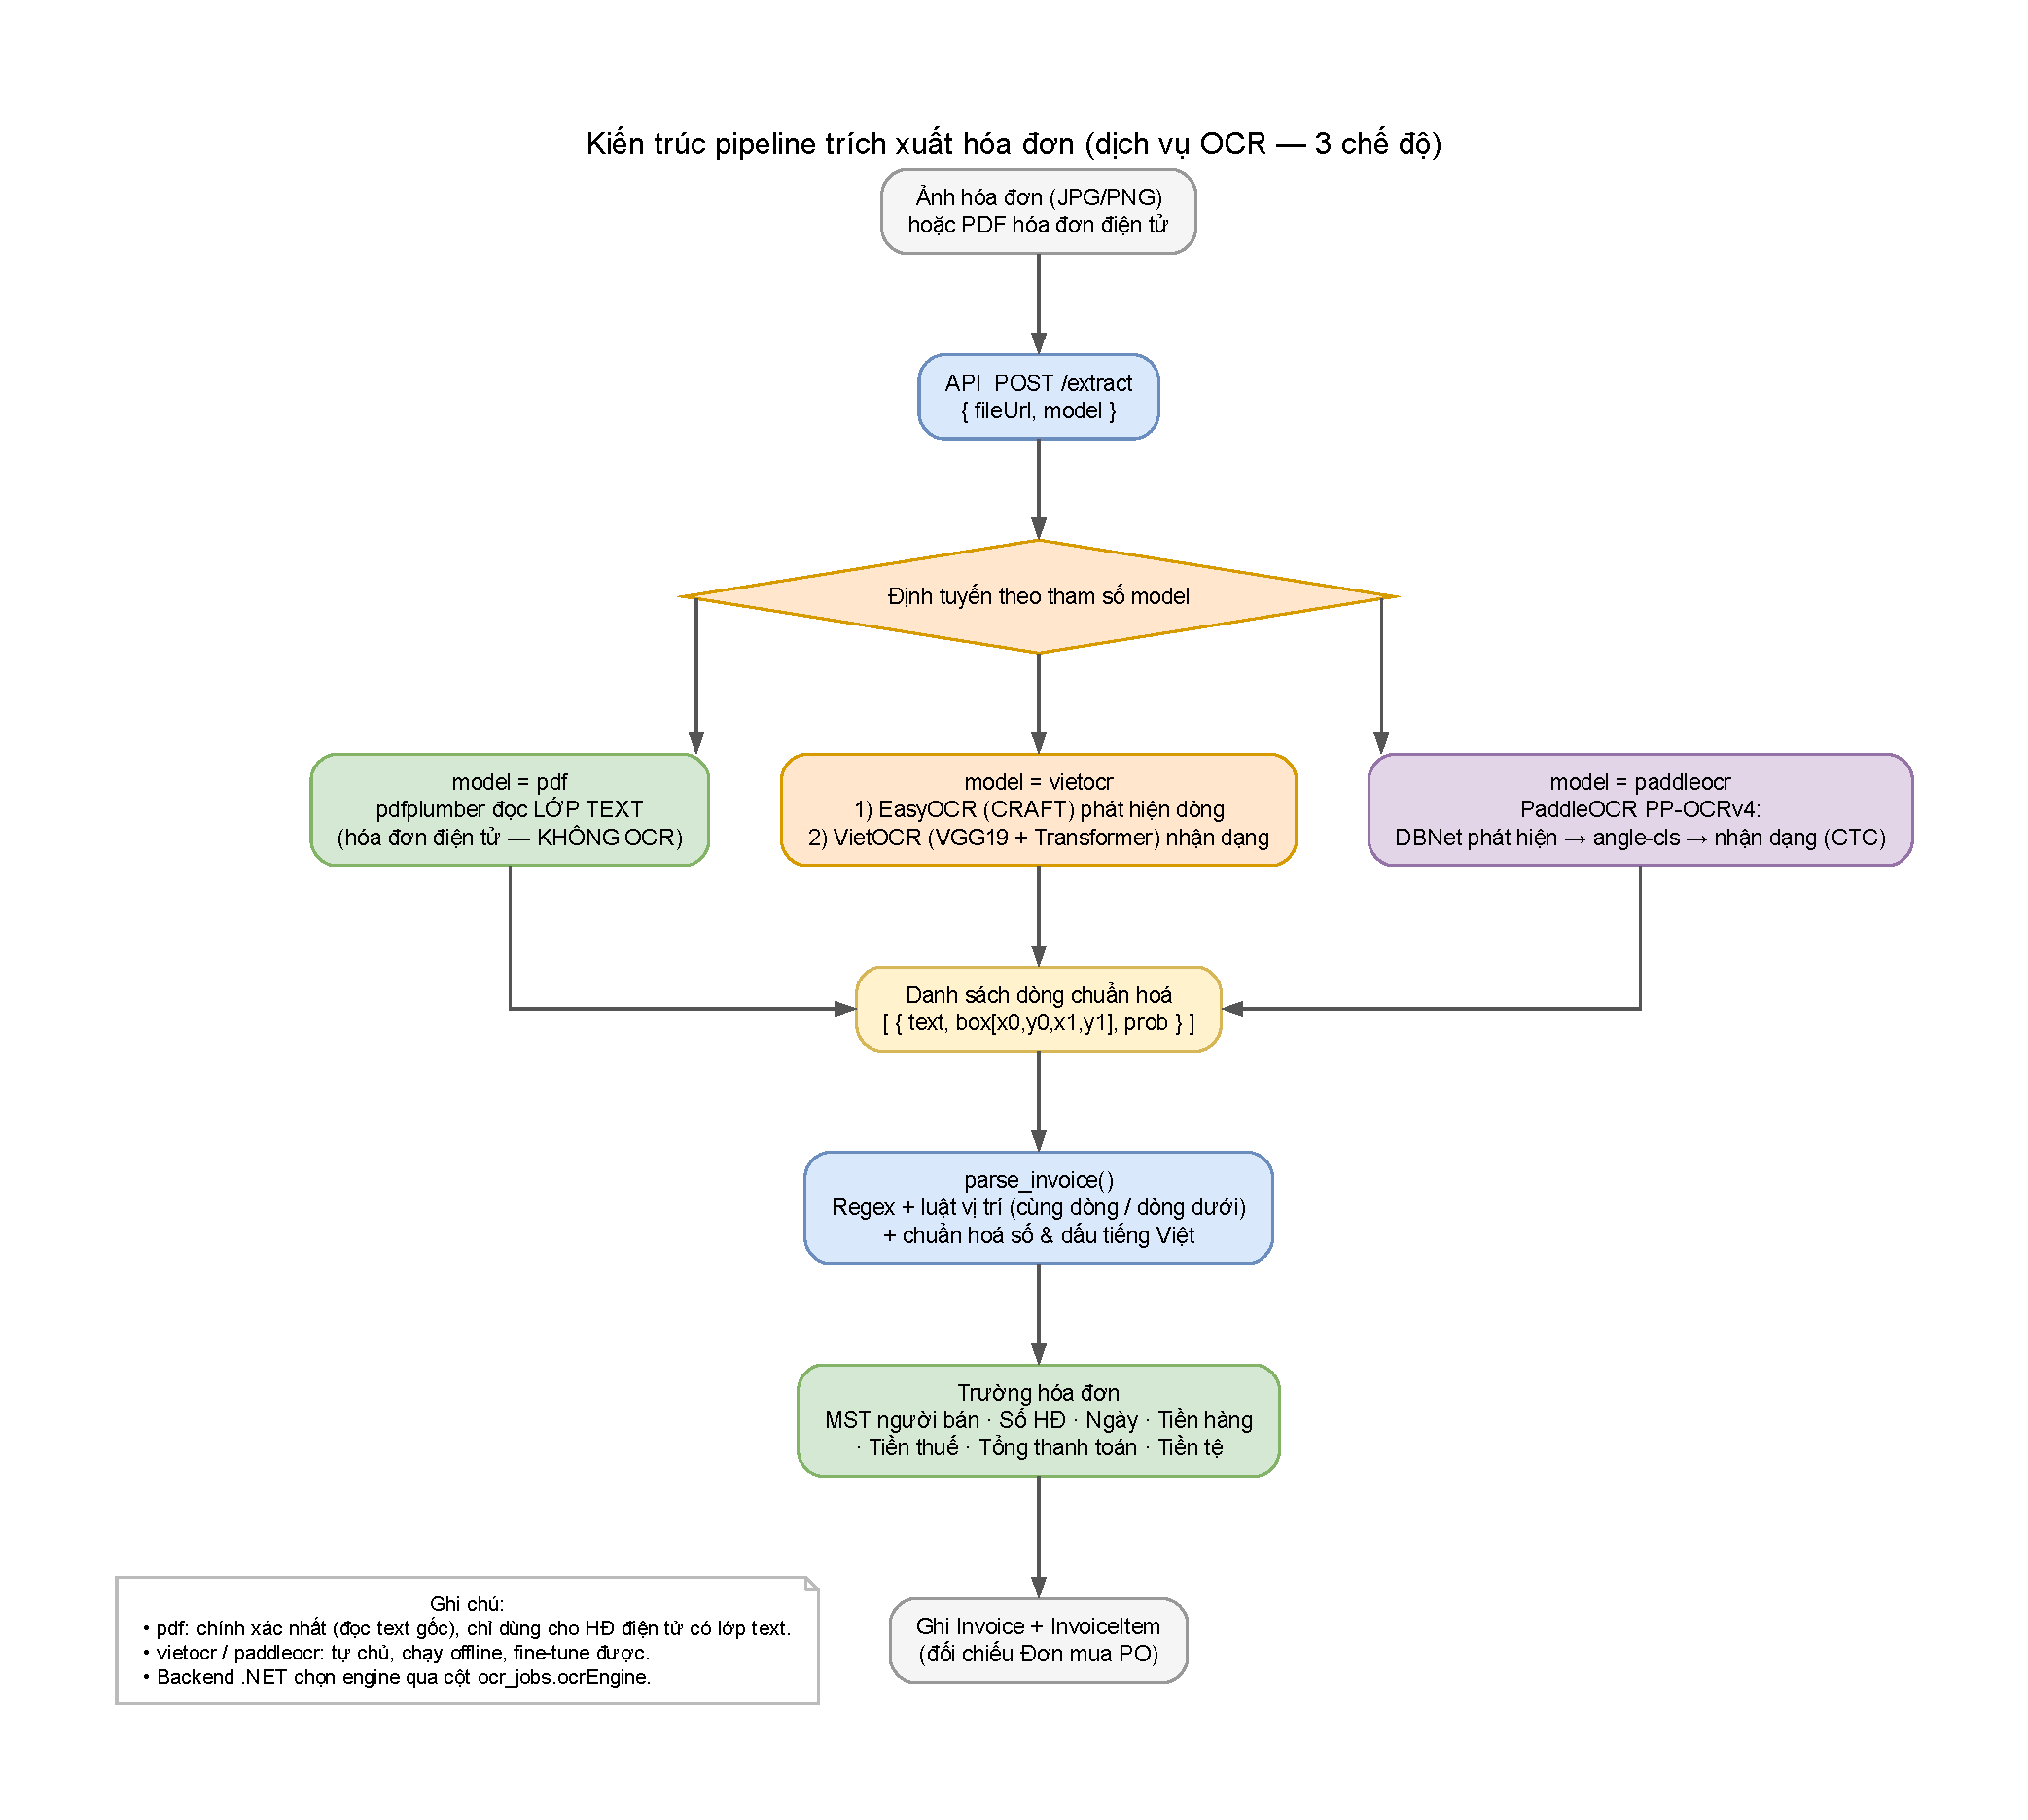
\includegraphics[width=\linewidth,height=0.5\textheight,keepaspectratio]{images/img27.pdf}
\caption*{\small Hình 4.20. Kiến trúc pipeline trích xuất hóa đơn của dịch vụ OCR}
\addcontentsline{lof}{figure}{Hình 4.20. Kiến trúc pipeline trích xuất hóa đơn của dịch vụ OCR}
\end{figure}
\subsubsection*{b) Cơ sở lý thuyết các mô hình}
\textbf{VietOCR} (vgg\_transformer, chỉ nhận dạng): CNN VGG19 trích đặc trưng ảnh dòng rồi Transformer encoder–decoder (seq2seq + attention) sinh từng ký tự theo từ điển tiếng Việt — đọc dấu thanh rất tốt nhưng buộc ghép một bộ phát hiện bên ngoài. \textbf{PaddleOCR} (PP-OCRv4, hợp nhất phát hiện + nhận dạng): DBNet (Differentiable Binarization) tách vùng chữ gọn, phân loại góc xoay dòng, rồi SVTR\_LCNet (huấn luyện GTC = CTC + NRTR) nhận dạng theo bảng ký tự \texttt{dict\_vi.txt} (137 ký tự) — một bộ công cụ, fine-tune được cả hai tầng, nhẹ, chạy offline. \textbf{EasyOCR (CRAFT)}: pipeline \texttt{vietocr} chỉ mượn CRAFT để cắt dòng; vì CRAFT không được fine-tune trên hóa đơn nên trở thành nút cổ chai — cũng là lý do thử biến thể hybrid \texttt{paddledet\_viet} ở mục h.

\subsubsection*{c) Dữ liệu, huấn luyện và luồng xử lý}
Vì không có sẵn dữ liệu hóa đơn thật đã gán nhãn, đề tài tự sinh dữ liệu hóa đơn GTGT tiếng Việt tổng hợp (synthetic): script tự render hóa đơn và tự ghi tọa độ + nội dung từng ô chữ, nên xuất được cả nhãn phát hiện (det) lẫn nhận dạng (rec) mà không cần gán tay, kèm bảng ký tự \texttt{dict\_vi.txt}. Dữ liệu được random đa dạng bố cục và tăng cường cho ``giống thật'' (nền giấy, nghiêng/méo, nhiễu, nén JPEG, dấu mộc đỏ, chữ ký tay); mọi phép biến hình đều kéo theo tọa độ box nên nhãn luôn khớp. Quy mô mặc định 400–500 hóa đơn, chia train/val 90/10; cả hai mô hình đều fine-tune từ trọng số pretrained (transfer learning) để hội tụ nhanh. Cấu hình thật (đọc từ config.yml):

\begin{center}{\small\singlespacing\renewcommand{\arraystretch}{1.3}
\begin{tabular}{|>{\raggedright\arraybackslash}p{\dimexpr0.16\linewidth-2\tabcolsep-\arrayrulewidth\relax}|>{\raggedright\arraybackslash}p{\dimexpr0.35\linewidth-2\tabcolsep-\arrayrulewidth\relax}|>{\raggedright\arraybackslash}p{\dimexpr0.13\linewidth-2\tabcolsep-\arrayrulewidth\relax}|>{\raggedright\arraybackslash}p{\dimexpr0.09\linewidth-2\tabcolsep-\arrayrulewidth\relax}|>{\raggedright\arraybackslash}p{\dimexpr0.27\linewidth-2\tabcolsep-\arrayrulewidth\relax}|}
\hline
\textbf{Mô hình} & \textbf{Thuật toán / Khởi tạo} & \textbf{Epoch} & \textbf{Batch} & \textbf{Optimizer / LR} \\ \hline
VietOCR (rec) & VGG19 + Transformer, từ vgg\_\allowbreak{}transformer & 20\,000 iters & 32 & mặc định VietOCR \\ \hline
PaddleOCR rec & SVTR\_\allowbreak{}LCNet + GTC(CTC+NRTR), từ PP-OCRv4 & 80 & 64 & Adam + Cosine, lr 0,001 \\ \hline
PaddleOCR det & DBNet, từ PP-OCRv4 det & 150 & 8 & lr 0,001 \\ \hline
\end{tabular}}\end{center}
\textbf{Luồng xử lý. }Pipeline vietocr: ảnh $\rightarrow$ EasyOCR/CRAFT phát hiện dòng $\rightarrow$ cắt dòng $\rightarrow$ VietOCR (VGG19 $\rightarrow$ Transformer) $\rightarrow$ text. Pipeline paddleocr: ảnh $\rightarrow$ DBNet $\rightarrow$ phân loại góc $\rightarrow$ SVTR\_LCNet $\rightarrow$ text. Cả hai gộp về danh sách dòng, đưa vào hàm bóc tách trường và ghi Invoice/InvoiceItem để đối chiếu PO.

\textbf{Kết quả huấn luyện PaddleOCR (số thật từ train.log). }Với nhận dạng (rec), loss giảm nhanh về gần 0 quanh bước \textasciitilde{}2\,500, trên tập val accuracy toàn chuỗi đạt 0,9964 (99,64\%) và norm\_edit\_dis 0,9992 tại epoch 41. Với phát hiện (det), hmean tốt nhất trên val chỉ đạt 0,2298 — cho thấy phát hiện bố cục trên dữ liệu synthetic còn yếu; khuyến nghị bổ sung 50–150 hóa đơn thật gán bằng PPOCRLabel, hoặc kết hợp detector pretrain với recognizer đã fine-tune.

\begin{figure}[htbp]\centering
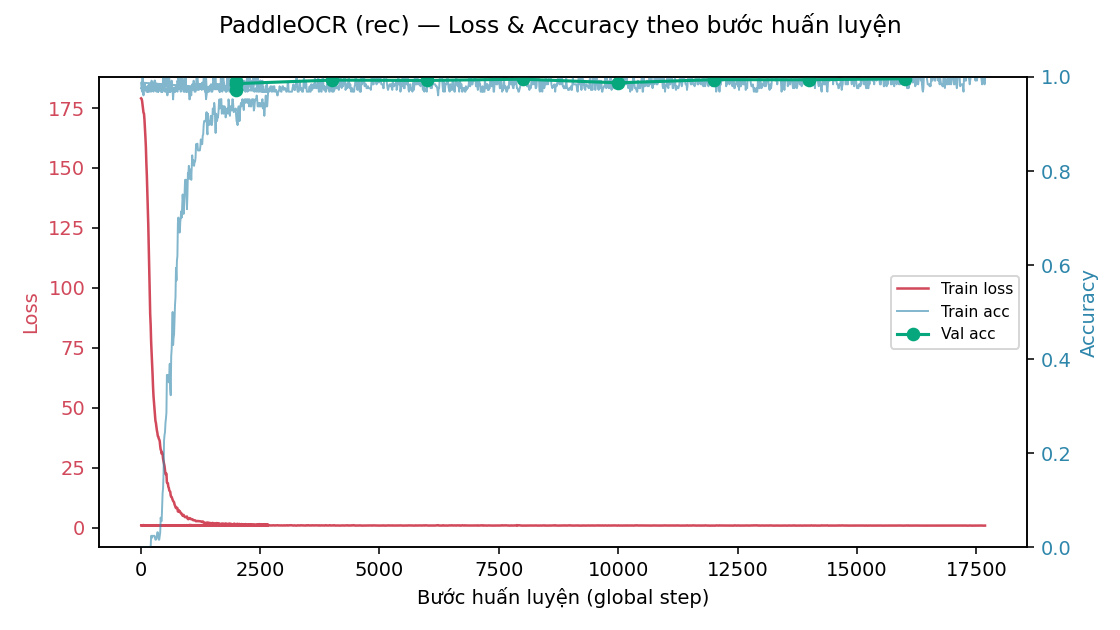
\includegraphics[width=\linewidth,height=0.42\textheight,keepaspectratio]{images/img29.png}
\caption*{\small Hình 4.21. Đường cong huấn luyện PaddleOCR (rec): loss và accuracy theo bước}
\addcontentsline{lof}{figure}{Hình 4.21. Đường cong huấn luyện PaddleOCR (rec)}
\end{figure}
\subsubsection*{d) So sánh và đánh giá ba engine}
Ba engine (EasyOCR, VietOCR, PaddleOCR) được đánh giá trên cùng tập val 300 mẫu với các chỉ số: Seq-acc (đọc đúng toàn chuỗi), Char-acc (1 $-$ CER), NED, CER<0,1 và độ trễ (ms/ảnh, đo trên CPU):

\begin{center}{\small\singlespacing\renewcommand{\arraystretch}{1.25}
\begin{tabular}{|>{\raggedright\arraybackslash}p{\dimexpr0.30\linewidth-2\tabcolsep-\arrayrulewidth\relax}|c|c|c|c|c|}
\hline
\textbf{Cấu hình} & \textbf{Seq-acc} & \textbf{Char-acc} & \textbf{NED} & \textbf{CER<0,1} & \textbf{ms/ảnh} \\ \hline
VietOCR gốc (trước) & 0,870 & 0,976 & 0,977 & 0,903 & - \\ \hline
VietOCR fine-tune (sau) & 1,000 & 1,000 & 1,000 & 1,000 & 317 \\ \hline
PaddleOCR gốc (trước) & 0,463 & 0,882 & 0,882 & 0,513 & - \\ \hline
PaddleOCR fine-tune (sau) & 0,893 & 0,967 & 0,968 & 0,913 & 65 \\ \hline
EasyOCR (baseline) & 0,510 & 0,811 & 0,818 & 0,613 & 156 \\ \hline
Ensemble (bỏ phiếu) & 0,920 & 0,974 & 0,974 & 0,933 & - \\ \hline
Oracle (best-of-3, chặn trên) & 1,000 & - & - & - & - \\ \hline
\end{tabular}}\end{center}
\begin{figure}[htbp]\centering
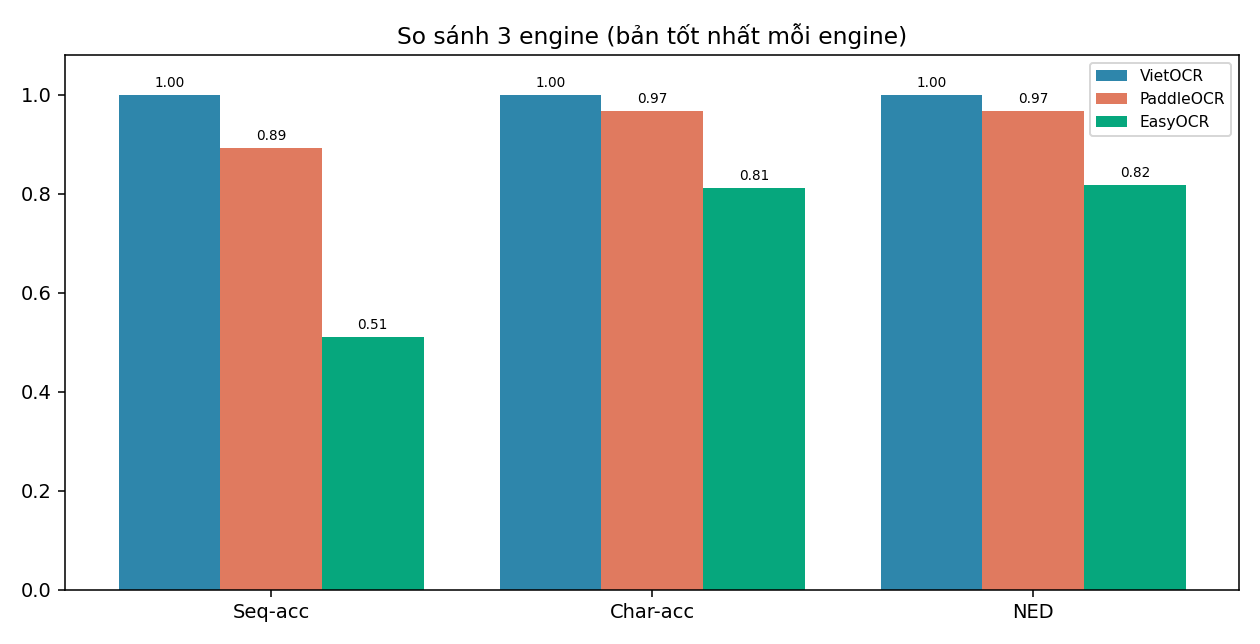
\includegraphics[width=\linewidth,height=0.42\textheight,keepaspectratio]{images/img31.png}
\caption*{\small Hình 4.22. So sánh ba engine theo Seq-acc / Char-acc / NED (tập val 300 mẫu)}
\addcontentsline{lof}{figure}{Hình 4.22. So sánh ba engine theo Seq-acc / Char-acc / NED}
\end{figure}
\textbf{Nhận xét. }(1) Fine-tune có tác động lớn: Seq-acc VietOCR tăng 0,870 $\rightarrow$ 1,000; PaddleOCR tăng 0,463 $\rightarrow$ 0,893 (PaddleOCR gốc pretrain tiếng Trung nên hưởng lợi nhiều nhất). (2) Về độ chính xác nhận dạng, VietOCR fine-tune đứng đầu (đúng 300/300 mẫu), trên PaddleOCR (0,893) và EasyOCR (0,510). (3) Về tốc độ, PaddleOCR nhanh nhất (65 ms/ảnh, nhanh hơn VietOCR \textasciitilde{}4,9 lần) và hợp nhất det+rec. Về \textbf{tính bổ trợ}: trong 300 mẫu không có mẫu nào cả ba cùng sai; ``chỉ VietOCR đúng'' = 24, ``chỉ PaddleOCR/chỉ EasyOCR đúng'' = 0, nên bỏ phiếu ba engine (0,920) còn thấp hơn VietOCR đơn lẻ (1,000) — với bài toán này dùng một engine mạnh hợp lý hơn là bỏ phiếu.

\subsubsection*{e) Lựa chọn mô hình}
\textbf{Vì sao chọn PaddleOCR thay vì kết hợp EasyOCR + VietOCR. }Phương án EasyOCR + VietOCR có recognizer rất chính xác nhưng vướng ba nhược điểm: tầng phát hiện CRAFT không được fine-tune (nút cổ chai), phải nạp hai bộ công cụ (nặng), và chậm nhất (317 ms/ảnh). PaddleOCR là một bộ công cụ hợp nhất, fine-tune được cả DBNet lẫn recognizer trên cùng dataset tự gán nhãn, nhẹ và nhanh nhất (65 ms/ảnh). Vì vậy PaddleOCR được chọn làm engine tự chủ mặc định; VietOCR giữ làm lựa chọn khi cần độ chính xác cao nhất; biến thể hybrid \texttt{paddledet\_viet} kết hợp điểm mạnh hai bên. Toàn bộ đều là giải pháp tự chủ, chạy offline, không phụ thuộc API bên ngoài.

\subsubsection*{f) Thuật toán bóc tách cấu trúc hóa đơn kháng nghiêng (deskew)}
\textbf{Đặt vấn đề. }Tầng OCR chỉ trả về danh sách ô văn bản kèm hộp bao, chưa phải dữ liệu có cấu trúc. Để dựng lại các trường (số hóa đơn, ngày, MST, các dòng tiền) và bảng chi tiết, hệ thống phải gom ô về đúng hàng và cột theo tọa độ. Ảnh chụp điện thoại thường nghiêng vài độ; khi đó độ lệch tung độ giữa mép trái–phải của bảng vượt quá chiều cao một dòng, khiến gom theo y gộp nhầm hai dòng liền kề. Đề tài đề xuất thuật toán hai pha khắc phục bằng hình học – thống kê, chạy sau tầng OCR và không cần huấn luyện.

\textbf{Pha A – Ước lượng và khử nghiêng. }Các ô thuộc hàng tiêu đề bảng (STT, Tên hàng, ĐVT, SL, Đơn giá, Thành tiền) vốn nằm trên cùng một phương ngang. Thuật toán khớp một đường thẳng qua tâm các ô này bằng bình phương tối thiểu; hệ số góc $a$ chính là độ nghiêng ($\theta$ = arctan $a$), rồi áp phép trượt (shear) ngược trên trục tung: $a = \Sigma(x_i - \bar{x})(y_i - \bar{y}) / \Sigma(x_i - \bar{x})^2$ và $y' = y - a\cdot x_i$. Sau đó mọi ô cùng một dòng vật lý có $y'$ xấp xỉ bằng nhau. Nếu $|a| < \varepsilon$ (ảnh vốn thẳng) thì bỏ qua bước trừ, bảo đảm bất biến với ảnh không nghiêng.

\textbf{Pha B – Tái tạo bảng theo cụm tọa độ. }Trên hệ tọa độ đã nắn thẳng: (1) xác định biên bảng giữa hàng tiêu đề và dòng ``Tổng/Thuế''; (2) gom dòng bằng phân cụm một chiều theo $y'$ với ngưỡng 0,6 lần chiều cao dòng trung vị; (3) gán mỗi ô vào cột có tâm hoành độ gần nhất (cột số chọn ô gần tâm cột nhất để tránh dính con số); (4) ghép mỗi cụm thành một dòng hàng và loại dòng rác. Độ phức tạp tổng thể $O(n\log n)$, bộ nhớ $O(n)$ với $n$ là số ô OCR. Trên hóa đơn thử nghiệm bị nghiêng, thuật toán tách đúng 7/7 dòng hàng, trong khi gom theo y thô chỉ nhận 3 hàng do bị dồn — thuần hình học, không cần mạng nơ-ron.

\begin{figure}[htbp]\centering
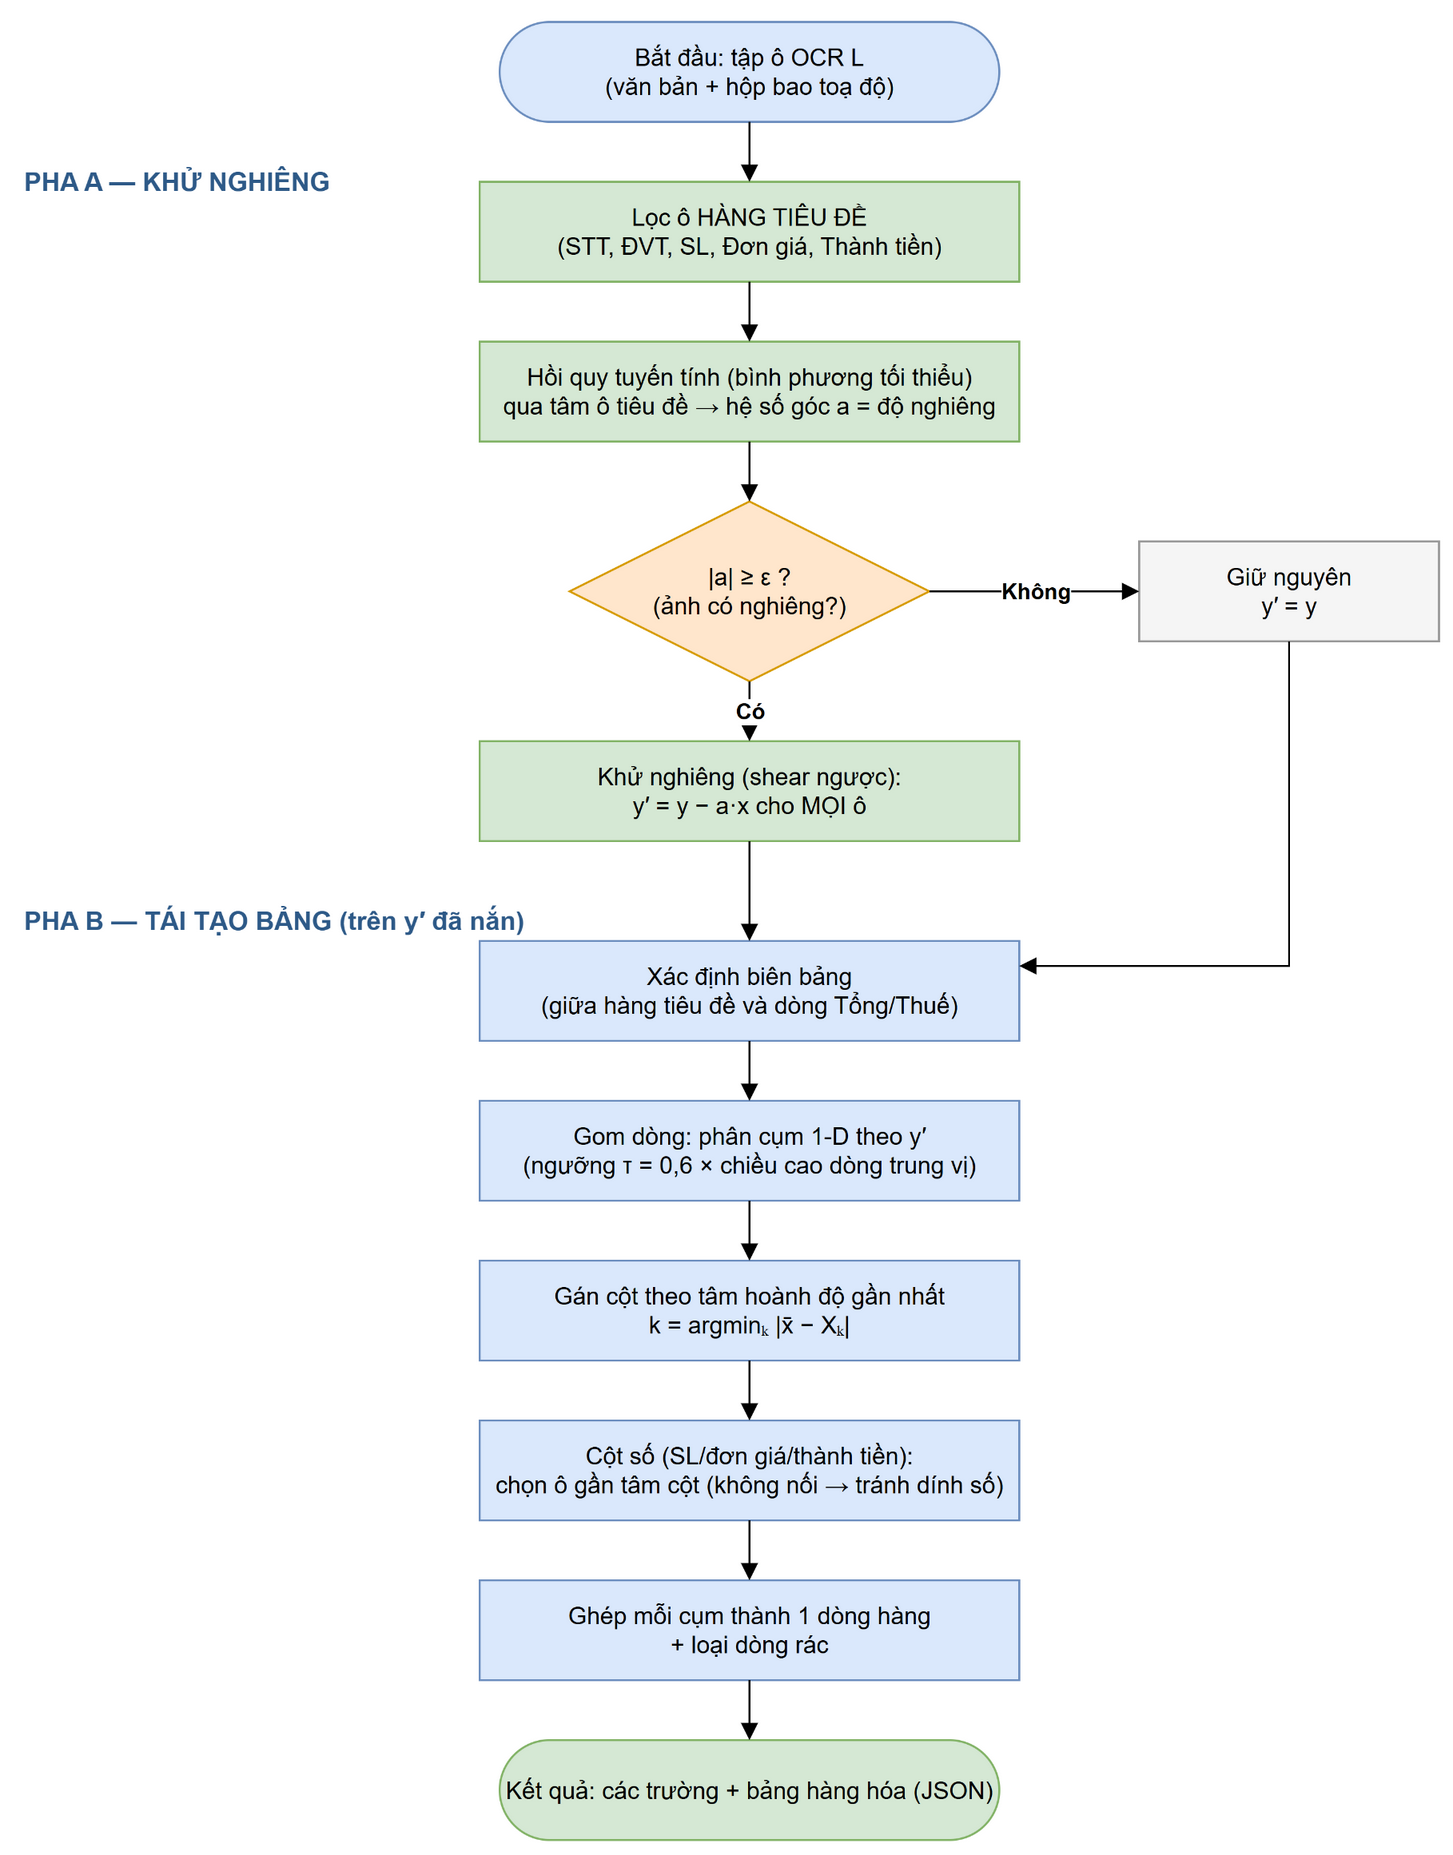
\includegraphics[width=\linewidth,height=0.42\textheight,keepaspectratio]{images/img34.png}
\caption*{\small Hình 4.23. Sơ đồ khối thuật toán bóc tách hóa đơn kháng nghiêng (deskew)}
\addcontentsline{lof}{figure}{Hình 4.23. Sơ đồ khối thuật toán bóc tách hóa đơn kháng nghiêng}
\end{figure}
\subsubsection*{g) Tổng hợp luồng xử lý AI end-to-end}
Hình 4.24 tổng hợp toàn bộ luồng từ ảnh đầu vào đến JSON đầu ra. (1) Đầu vào ảnh hóa đơn (JPG/PNG); (2) tiền xử lý chuẩn hóa RGB; (3) rẽ nhánh theo \texttt{ocrEngine} giữa ba engine tự chủ, đều đi qua lớp Phát hiện rồi Nhận dạng; (4) Phát hiện: CRAFT (vietocr) hoặc DBNet + phân loại góc (paddleocr); (5) Nhận dạng: VietOCR hoặc SVTR\_LCNet tạo danh sách ô OCR (text, box, prob). (6) Hậu xử lý biến ô rời rạc thành dữ liệu có cấu trúc qua năm bước: \textcircled{\scriptsize 1} khử nghiêng ($y' = y - a\cdot x$, bước ĐẦU TIÊN), \textcircled{\scriptsize 2} gom hàng theo $y'$, \textcircled{\scriptsize 3} trích trường bằng nhãn + regex, \textcircled{\scriptsize 4} trích bảng theo tâm cột, \textcircled{\scriptsize 5} chuẩn hóa số và bù tổng. (7) Đầu ra JSON (fields, lineItems, confidence) được backend .NET lưu vào Invoice/InvoiceItem và hiển thị ở màn hình xác nhận.

\begin{figure}[htbp]\centering
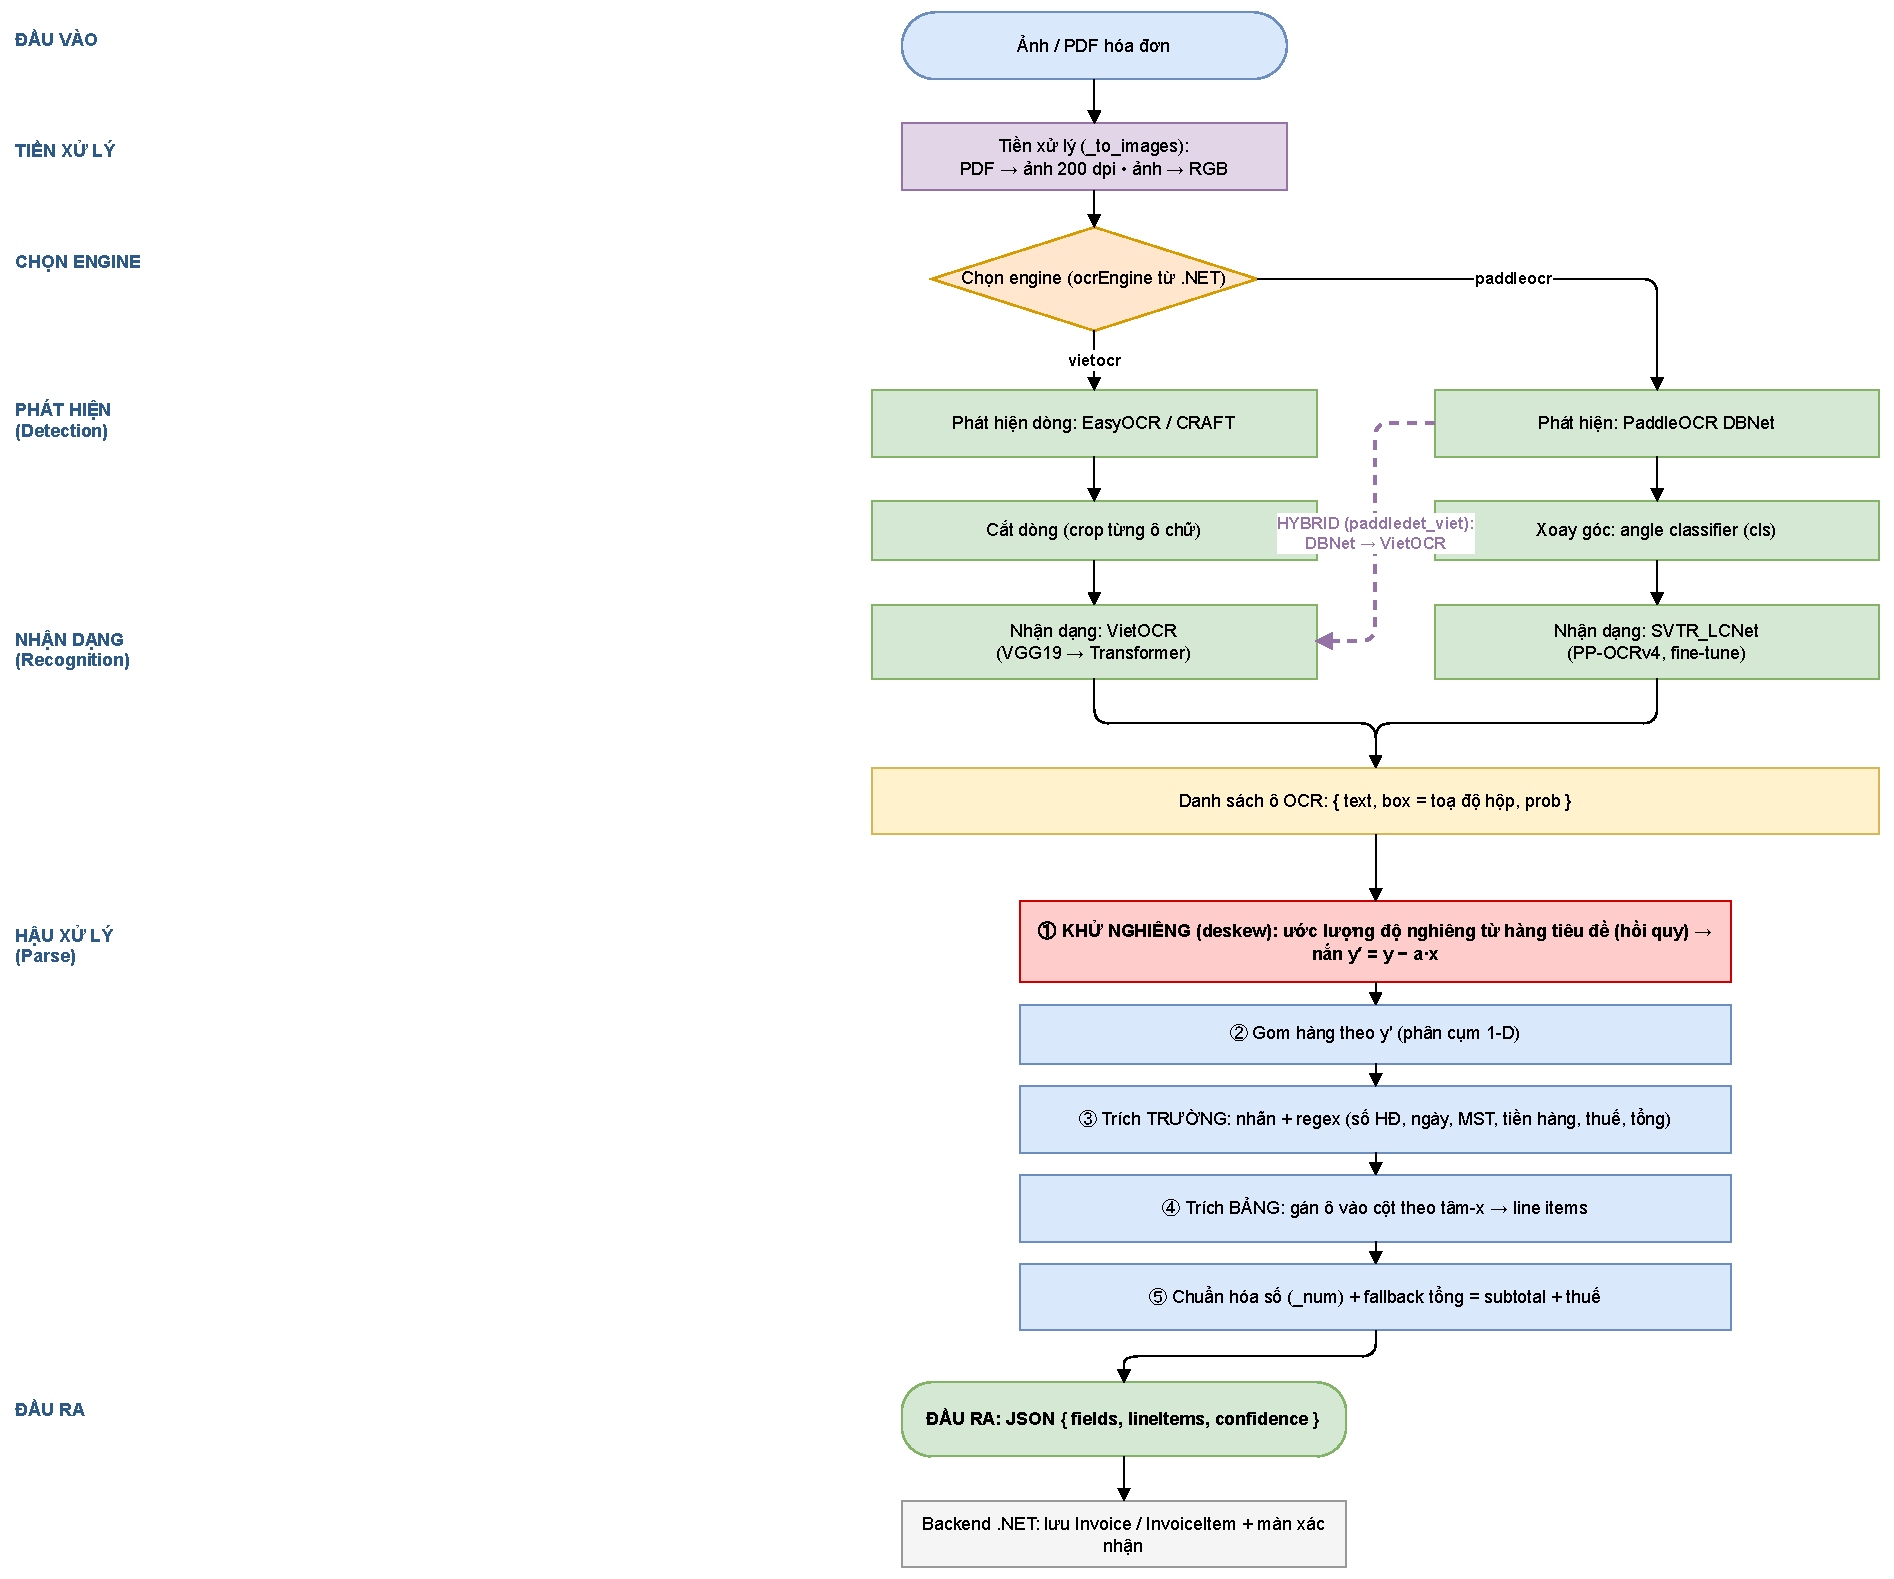
\includegraphics[width=\linewidth,height=0.5\textheight,keepaspectratio]{images/img35.pdf}
\caption*{\small Hình 4.24. Luồng xử lý AI end-to-end của dịch vụ OCR: các lớp xử lý và vị trí bước khử nghiêng}
\addcontentsline{lof}{figure}{Hình 4.24. Luồng xử lý AI end-to-end của dịch vụ OCR}
\end{figure}
\subsubsection*{h) Biến thể hybrid: Paddle DBNet (phát hiện) + VietOCR (nhận dạng)}
\textbf{Ý tưởng \& cơ chế. }VietOCR cho độ chính xác nhận dạng cao nhất, còn DBNet của PaddleOCR (đã fine-tune) phát hiện tốt hơn CRAFT của EasyOCR. Biến thể hybrid (\texttt{paddledet\_viet}) ghép hai điểm mạnh: DBNet phát hiện dòng, sau đó phép biến đổi phối cảnh đưa mỗi vùng (đa giác bốn điểm của DBNet) về ảnh dòng nằm ngang rồi giao VietOCR nhận dạng. Kết quả trả về cùng định dạng danh sách ô nên tái dùng nguyên vẹn bộ hậu xử lý ở mục f, g.

\textbf{Đánh đổi và lựa chọn. }So sánh \texttt{paddleocr} với \texttt{paddledet\_viet} là một ablation giữ nguyên detector, chỉ thay recognizer. Khác biệt của hybrid nằm ở tầng phát hiện: DBNet cắt dòng ổn định hơn CRAFT nên khi chạy end-to-end trên hóa đơn cả trang, hybrid được kỳ vọng vượt pipeline vietocr. Bù lại, hybrid phải nạp đồng thời hai framework (PaddlePaddle + PyTorch) nên tốn bộ nhớ và chậm hơn, triển khai phức tạp hơn PaddleOCR hợp nhất. Vì vậy hệ thống chọn PaddleOCR làm engine mặc định, còn hybrid là tùy chọn phục vụ đối chiếu và tình huống ưu tiên độ chính xác nhận dạng hơn tốc độ.

\phantomsection
\subsection*{4.4.2. Khảo sát các giải pháp AI OCR khác và lý do lựa chọn}
\addcontentsline{toc}{subsection}{4.4.2. Khảo sát các giải pháp AI OCR khác và lý do lựa chọn}
Bóc tách hóa đơn bằng AI là bài toán đã trưởng thành, có nhiều giải pháp thương mại và mã nguồn mở. Trước khi tự xây dựng engine, nhóm đã khảo sát ba nhóm giải pháp phổ biến để làm căn cứ lựa chọn (số liệu giá tham khảo tại thời điểm khảo sát 07/2026); bảng tổng hợp và bảng xếp hạng công khai ở cuối mục.

\textbf{a) Nhóm dịch vụ đám mây (Cloud OCR/IDP API).} Các API trả tiền theo lượt gọi, độ chính xác cao và không phải tự vận hành hạ tầng, nhưng dữ liệu phải gửi ra máy chủ bên thứ ba và chi phí tăng theo sản lượng:
\begin{itemize}[leftmargin=1.4em,itemsep=1pt,topsep=2pt]
  \item \textbf{Google Cloud Vision / Document AI}: giá cơ bản \textasciitilde{}1,5 USD/1.000 trang, bản trích cấu trúc (Document AI) cao hơn nhiều; miễn phí 1.000 đơn vị/tháng.
  \item \textbf{Azure AI Document Intelligence}: có mô hình hóa đơn dựng sẵn (prebuilt-invoice), \textasciitilde{}10 USD/1.000 trang; miễn phí 500 trang/tháng.
  \item \textbf{Amazon Textract}: DetectDocumentText \textasciitilde{}1,5 USD/1.000 trang, AnalyzeDocument (bảng/biểu mẫu) tới \textasciitilde{}65 USD/1.000 trang.
\end{itemize}

\textbf{b) Nhóm SDK thương mại cài tại chỗ.} Tiêu biểu là \textbf{ABBYY FineReader Engine} — bộ SDK OCR lâu đời, độ chính xác cao, chạy được on-premise (bảo mật tốt) nhưng chi phí bản quyền lớn và mô hình đóng, không tùy biến sâu cho hóa đơn tiếng Việt.

\textbf{c) Nhóm mã nguồn mở, tự triển khai.} Miễn phí, chạy offline, tùy biến và fine-tune được:
\begin{itemize}[leftmargin=1.4em,itemsep=1pt,topsep=2pt]
  \item \textbf{Tesseract}: engine mã nguồn mở lâu đời của Google; đọc tài liệu in tốt nhưng yếu với hóa đơn tiếng Việt bố cục phức tạp nếu không huấn luyện lại, và chậm hơn.
  \item \textbf{PaddleOCR} (Hình 4.25): bộ công cụ OCR nhẹ, hợp nhất phát hiện + nhận dạng, hỗ trợ 100+ ngôn ngữ, fine-tune được cả hai tầng, nhanh — đây là engine nhóm chọn, kết hợp thêm \textbf{VietOCR} (recognizer mạnh về dấu tiếng Việt) và bộ phát hiện CRAFT của EasyOCR.
\end{itemize}

\begin{figure}[htbp]\centering
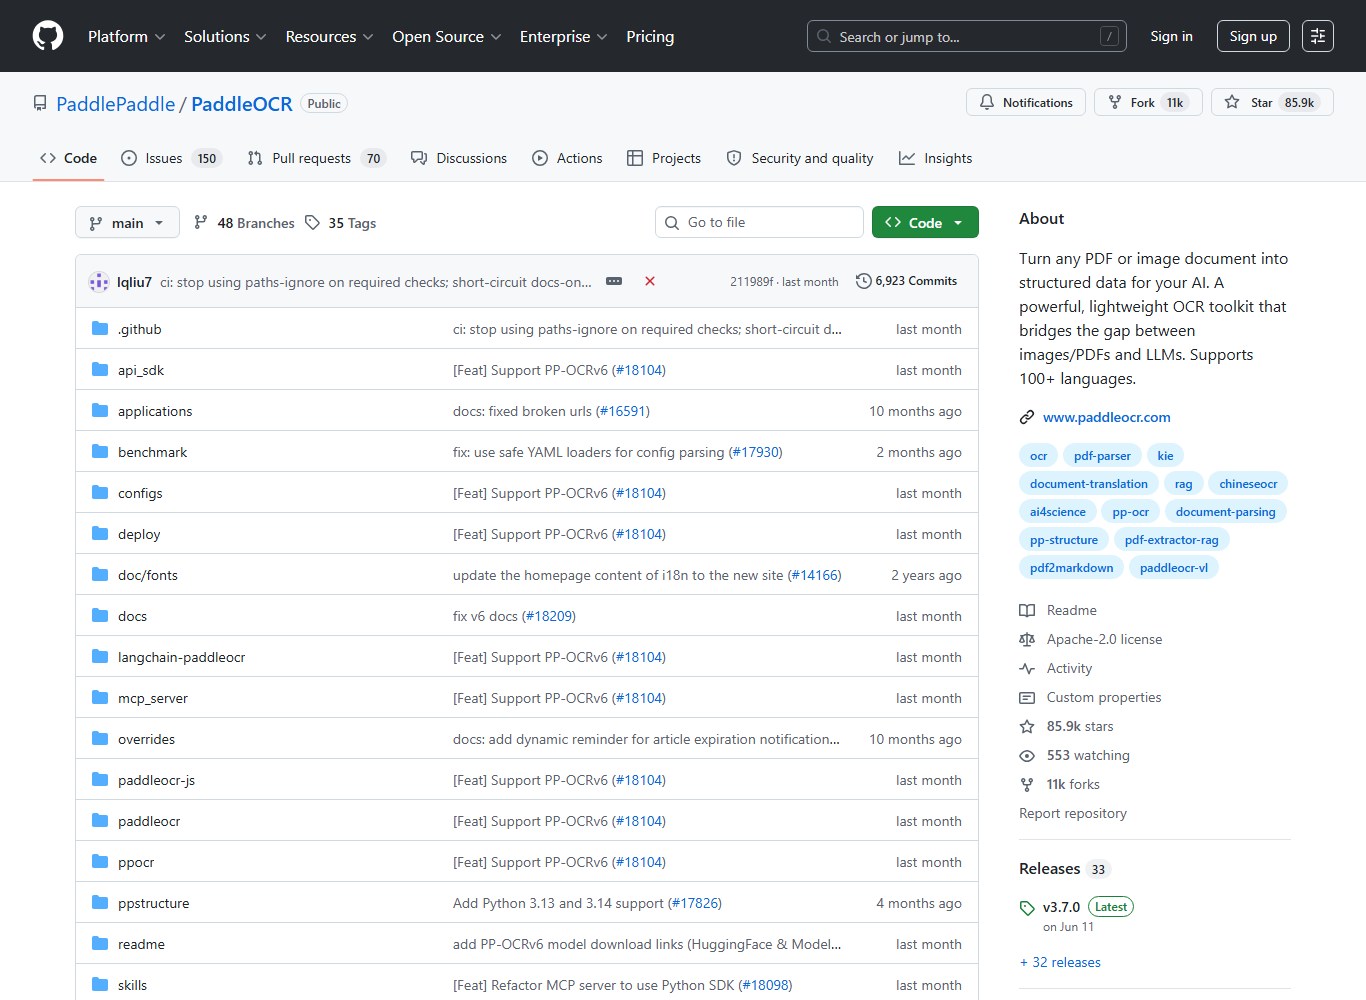
\includegraphics[width=\linewidth,height=0.34\textheight,keepaspectratio]{images/ocr_paddle.png}
\caption*{\small Hình 4.25. PaddleOCR (mã nguồn mở, Apache-2.0, \textasciitilde{}86k sao GitHub) -- engine nhóm lựa chọn}
\addcontentsline{lof}{figure}{Hình 4.25. PaddleOCR (mã nguồn mở) -- engine được chọn}
\end{figure}
\noindent\textit{\small Nguồn: \url{https://github.com/PaddlePaddle/PaddleOCR} (truy cập 07/2026).}

\textbf{Bảng xếp hạng, so sánh các giải pháp.} Nhóm chấm điểm theo các tiêu chí quan trọng với bài toán (đọc hóa đơn tiếng Việt trong hệ quản lý tòa nhà) và với yêu cầu của một đồ án tốt nghiệp:

\begin{landscape}\begin{center}{\footnotesize\singlespacing\renewcommand{\arraystretch}{1.25}
\begin{tabular}{|>{\raggedright\arraybackslash}p{3.1cm}|>{\raggedright\arraybackslash}p{2.3cm}|>{\raggedright\arraybackslash}p{2.6cm}|>{\raggedright\arraybackslash}p{2.6cm}|>{\raggedright\arraybackslash}p{2.5cm}|>{\raggedright\arraybackslash}p{2.5cm}|>{\raggedright\arraybackslash}p{2.4cm}|}
\hline
\textbf{Giải pháp} & \textbf{Loại} & \textbf{Độ chính xác HĐ tiếng Việt} & \textbf{Chi phí} & \textbf{Tự chủ / Offline \& bảo mật} & \textbf{Fine-tune trên dữ liệu riêng} & \textbf{Phù hợp đồ án} \\ \hline
Google Vision / Document AI & Cloud API & Cao & Trả theo lượt (\textasciitilde{}1,5–nhiều USD/1k trang) & Không (gửi HĐ lên cloud) & Hạn chế (không sở hữu model) & Thấp \\ \hline
Azure Document Intelligence & Cloud API & Cao & \textasciitilde{}10 USD/1k trang (invoice) & Không / có container trả phí & Custom model (trả phí) & Thấp \\ \hline
Amazon Textract & Cloud API & Cao & \textasciitilde{}1,5–65 USD/1k trang & Không & Không & Thấp \\ \hline
ABBYY FineReader & SDK thương mại & Cao & Bản quyền lớn & Có (on-prem) & Hạn chế (đóng) & Thấp \\ \hline
Tesseract & Mã nguồn mở & Trung bình–thấp & Miễn phí & Có & Có (khó) & Trung bình \\ \hline
\textbf{PaddleOCR (chọn)} & Mã nguồn mở & \textbf{Cao} (0,893 seq; 65 ms) & Miễn phí & \textbf{Có} & \textbf{Có (det+rec)} & \textbf{Rất phù hợp} \\ \hline
\textbf{VietOCR (chọn)} & Mã nguồn mở & \textbf{Rất cao} (1,000 seq) & Miễn phí & \textbf{Có} & \textbf{Có (rec)} & \textbf{Rất phù hợp} \\ \hline
\end{tabular}}\end{center}\end{landscape}
\noindent\textit{\small Nguồn số liệu giá: trang giá chính thức của Google Cloud Vision, Azure AI Document Intelligence và \url{https://aws.amazon.com/textract/pricing/} (07/2026); số liệu độ chính xác/tốc độ engine lấy từ thực nghiệm của nhóm ở mục 4.4.1.d.}

\textbf{Đối chiếu với bảng xếp hạng AI công khai (OmniDocBench).} Để tăng tính khách quan, nhóm đối chiếu lựa chọn của mình với bảng xếp hạng độc lập, công khai \textbf{OmniDocBench} (CVPR 2025, nhóm OpenDataLab) — benchmark chuẩn cho bài toán bóc tách tài liệu, chấm điểm end-to-end trên nhiều loại tài liệu và cập nhật liên tục cho cả mô hình mã nguồn mở lẫn thương mại. Đáng chú ý, \textbf{PaddleOCR — chính là họ engine đề tài sử dụng — hiện dẫn đầu bảng}: biến thể \texttt{PP-StructureV3} và các mô hình \texttt{PaddleOCR-VL} đạt điểm tổng cao nhất, vượt cả mô hình đa phương thức thương mại như GPT-5.2 hay Gemini~3~Pro. Trích một phần bảng xếp hạng (điểm \emph{Overall}, thang 100, 07/2026):

\begin{center}{\footnotesize\singlespacing\renewcommand{\arraystretch}{1.25}
\begin{tabular}{|c|>{\raggedright\arraybackslash}p{5.0cm}|>{\raggedright\arraybackslash}p{3.4cm}|c|}
\hline
\textbf{Hạng} & \textbf{Mô hình / công cụ} & \textbf{Loại} & \textbf{Overall} \\ \hline
1 & \textbf{PaddleOCR-VL-1.6} \textit{(họ PaddleOCR)} & Mã nguồn mở & \textbf{96,34} \\ \hline
2 & MinerU2.5-Pro & Mã nguồn mở & 95,75 \\ \hline
4 & \textbf{PaddleOCR-VL-1.5} \textit{(họ PaddleOCR)} & Mã nguồn mở & \textbf{94,93} \\ \hline
13 & Gemini 3 Pro \textit{(tham chiếu)} & VLM thương mại & 92,91 \\ \hline
\end{tabular}}\end{center}

\begin{figure}[htbp]\centering
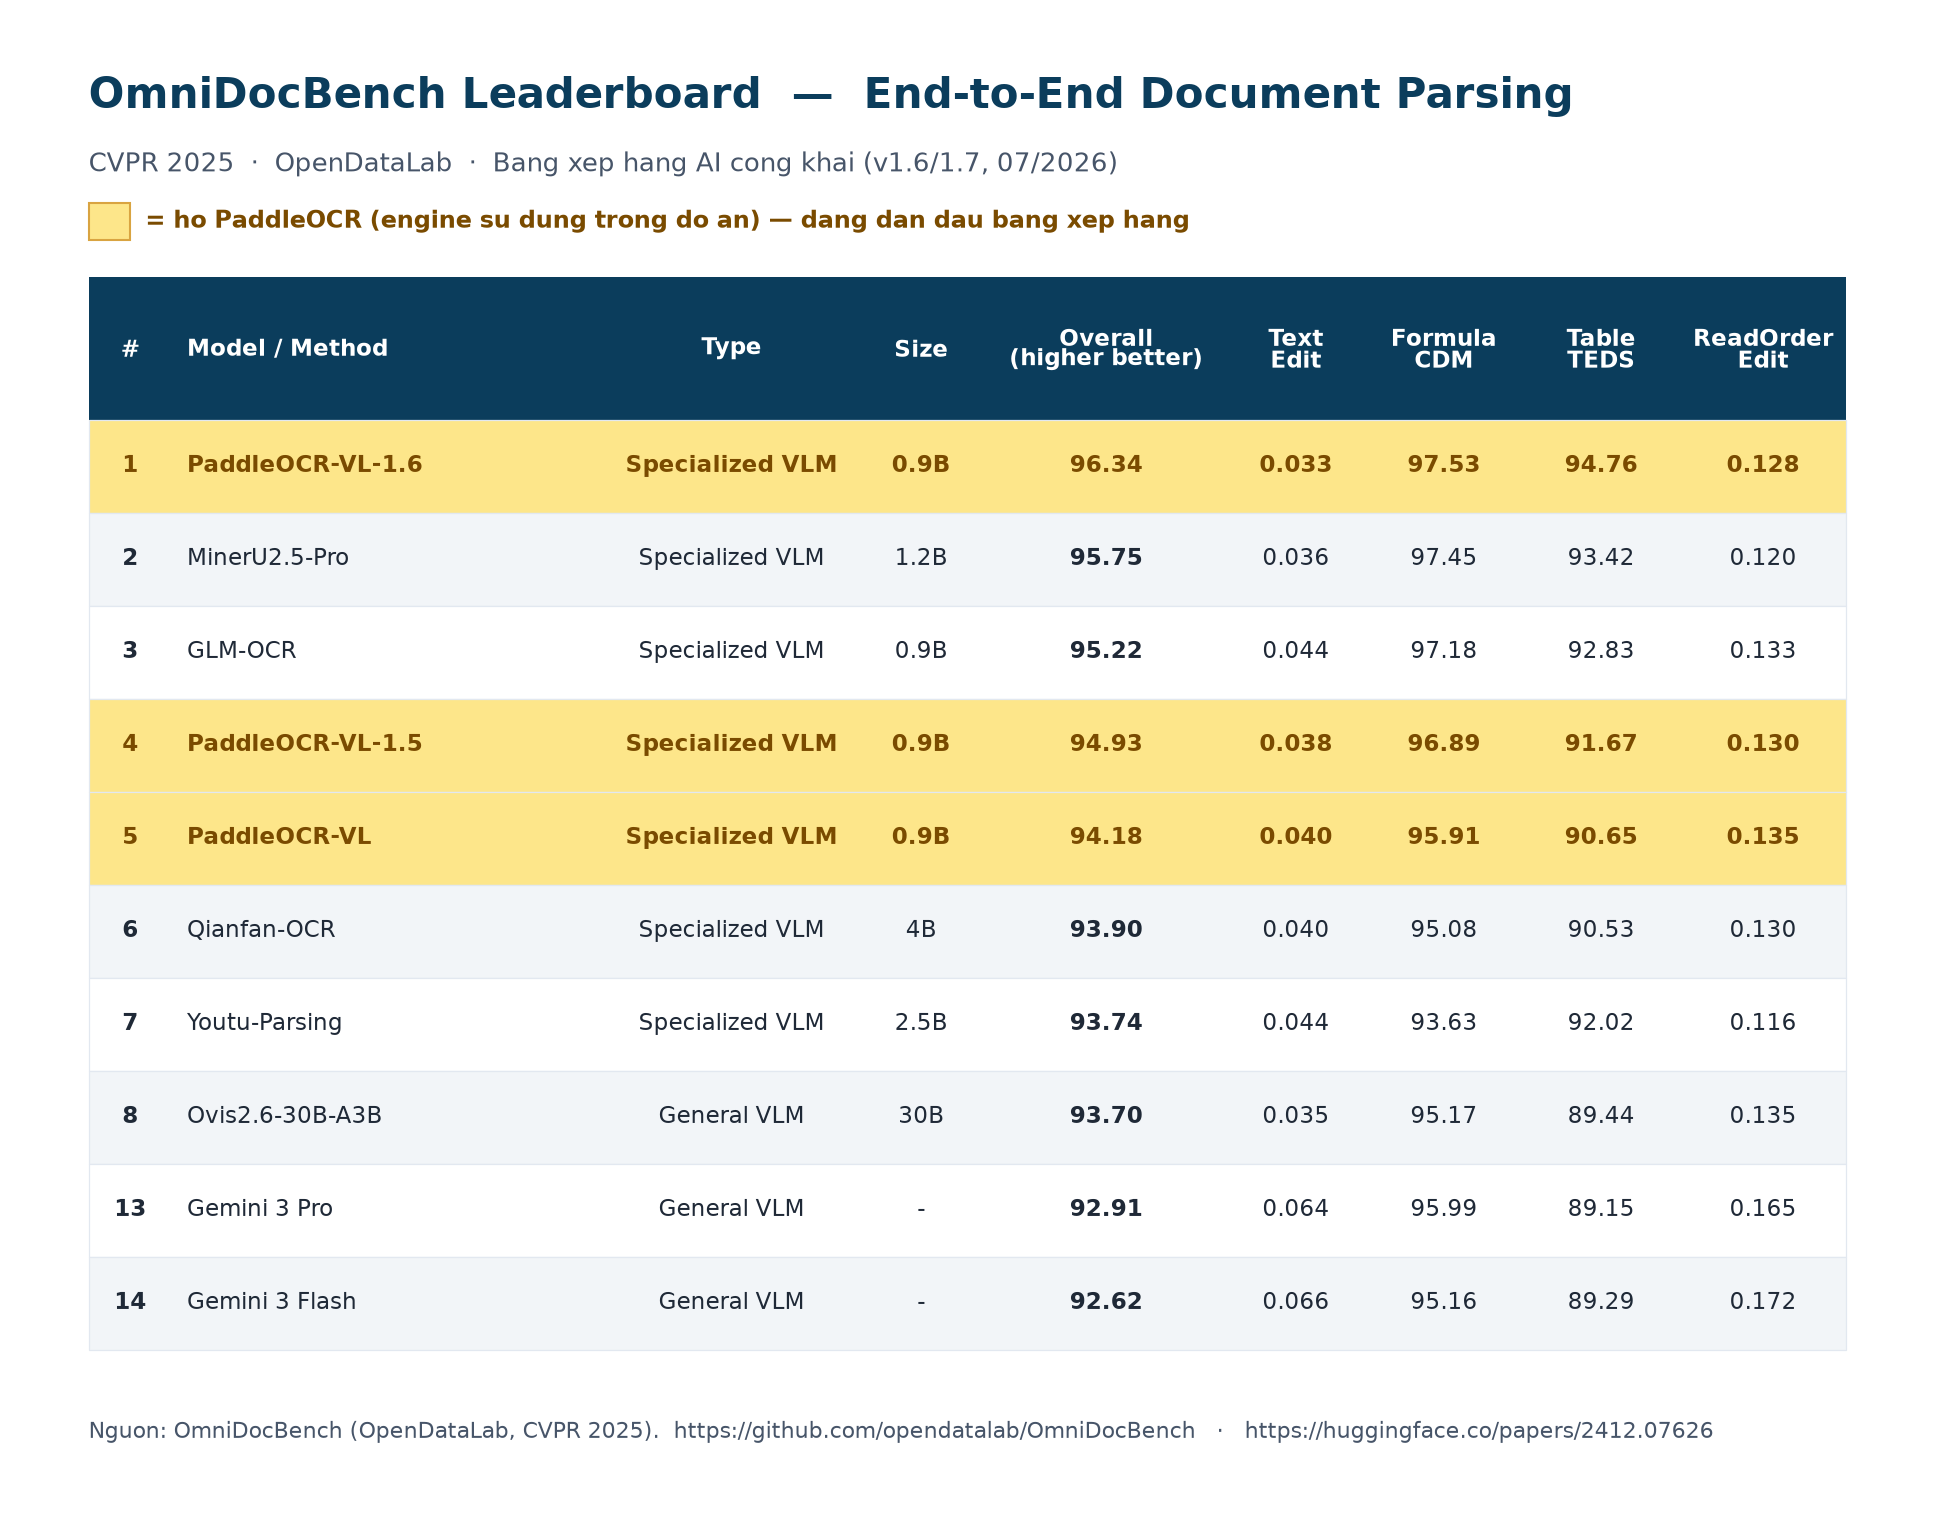
\includegraphics[width=\linewidth,height=0.34\textheight,keepaspectratio]{images/ocr_leaderboard_omnidocbench.png}
\caption*{\small Hình 4.26. Bảng xếp hạng AI công khai OmniDocBench (CVPR 2025) — họ engine PaddleOCR dẫn đầu}
\addcontentsline{lof}{figure}{Hình 4.26. Bảng xếp hạng AI công khai OmniDocBench — PaddleOCR dẫn đầu}
\end{figure}
\noindent\textit{\small Nguồn: OmniDocBench, OpenDataLab (CVPR 2025): \url{https://github.com/opendatalab/OmniDocBench}; \url{https://opendatalab.com/OmniDocBench} (truy cập 07/2026).}

\textbf{Lý do lựa chọn PaddleOCR + VietOCR (tự triển khai).} Trên cơ sở khảo sát, nhóm chọn hướng \emph{tự triển khai mã nguồn mở} thay vì API đám mây hay SDK thương mại, vì: \textbf{(1) Bảo mật} — hóa đơn chứa thông tin tài chính–thuế nhạy cảm, giải pháp tự triển khai chạy offline, dữ liệu không rời khỏi hệ thống; \textbf{(2) Chi phí} — miễn phí bản quyền, không phí theo lượt gọi (API đám mây \textasciitilde{}1,5–65 USD/1.000 trang); \textbf{(3) Fine-tune được trên dữ liệu tiếng Việt} — nhóm tự sinh dataset và fine-tune đạt 99,64\% (PaddleOCR) và 100\% (VietOCR), điều mà API/SDK đóng không cho phép; \textbf{(4) Chủ động}, không lệ thuộc Internet hay vendor lock-in; \textbf{(5) Đúng tinh thần đồ án} — thể hiện năng lực xây dựng, huấn luyện và đánh giá mô hình AI thay vì chỉ gọi dịch vụ có sẵn. Tóm lại, các giải pháp đám mây/thương mại chính xác và tiện nhưng đánh đổi chi phí, quyền riêng tư và khả năng tùy biến; hướng tự triển khai PaddleOCR + VietOCR đáp ứng tốt nhất các tiêu chí của đề tài.

\phantomsection


\phantomsection
\section*{4.5. Kết luận chương}
\addcontentsline{toc}{section}{4.5. Kết luận chương}
Chương 4 đã phân rã chi tiết ba nhóm chức năng của phân hệ Quản lý tài sản — Mua sắm, Vòng đời tài sản, Bảo trì \& Sự cố — mỗi nhóm với use case + đặc tả, sơ đồ luồng, biểu đồ tuần tự, sơ đồ trạng thái và ERD, bám sát mã nguồn và các chuẩn tham chiếu (Odoo, ITIL, Thông tư 200/133, BPMN). Ba nhóm liên thông chặt qua kho -- vật tư -- tài sản -- work order, tạo thành một phân hệ quản lý tài sản hoàn chỉnh và là đóng góp cá nhân của tác giả theo Điều 7.
